\documentclass[12pt,a4paper]{article}

\usepackage[margin=2.3cm]{geometry}
\usepackage{amsmath,amssymb,amsthm}
\usepackage{graphicx}
\usepackage{booktabs,multirow,array,tabularx}
\usepackage{algorithm,algpseudocode}
\usepackage[colorlinks=true,linkcolor=blue!60!black,
            citecolor=blue!60!black,urlcolor=blue!60!black]{hyperref}
\usepackage{xcolor,caption,subcaption}
\usepackage{setspace,enumitem,cite}
\usepackage{placeins}   %% \FloatBarrier
\usepackage{pgfplots,pgfplotstable}
\pgfplotsset{compat=1.18}
\usepackage{tikz}
\usetikzlibrary{shapes.geometric,arrows.meta,positioning,calc,decorations.pathreplacing}
%% Ensure figures never float past section boundaries
\let\oldsection\section
\renewcommand{\section}[1]{\FloatBarrier\oldsection{#1}}
\let\oldsubsection\subsection
\renewcommand{\subsection}[1]{\FloatBarrier\oldsubsection{#1}}

\setstretch{1.10}
\renewcommand{\arraystretch}{0.93}

\newtheorem{definition}{Definition}
\newtheorem{proposition}{Proposition}
\newtheorem{remark}{Remark}
\newtheorem{observation}{Observation}

%% --- Notation shortcuts ---
\newcommand{\Rset}{\mathbb{R}}
\newcommand{\sched}{\sigma}
\newcommand{\Tmin}{T_{\min}}
\newcommand{\Tmax}{T_{\max}}
\newcommand{\Tout}{T_{\mathrm{out}}}
\newcommand{\Cth}{C_{\mathrm{th}}}
\newcommand{\lext}{\lambda_{\mathrm{ext}}}
\newcommand{\lwin}{\lambda_{\mathrm{win}}}
\newcommand{\lij}{\lambda_{ij}}
\newcommand{\Qhvac}{Q_{\mathrm{hvac}}}
\newcommand{\csw}{c_{\mathrm{sw}}}
\newcommand{\Phvac}{P_{\mathrm{hvac}}}
\newcommand{\Jbar}{\bar{J}}
\newcommand{\SAR}{\text{SAR}}
\newcommand{\kWh}{\text{kWh}}
\newcommand{\Liz}[1]{\Lambda_{\mathrm{iz},#1}}
\newcommand{\Tiz}[1]{T_{\mathrm{iz},#1}}
\newcommand{\Qiz}[1]{Q_{\mathrm{iz},#1}}
\newcommand{\taup}{\tau^{+}}
\newcommand{\taum}{\tau^{-}}

%% ============================================================
\begin{document}

\title{\textbf{Constrained Optimal Binary HVAC Scheduling over an
Infinite Time Horizon in Saudi Residential Buildings: A Hybrid
Rule-Based Reinforcement Learning Framework}}

\author{
  Hamzah Faraj\\[3pt]
  Department of Science and Technology, Ranyah College,\\
  Taif University, Taif 21944, Saudi Arabia\\[3pt]
 \thanks{Corresponding author: f.hamzah@tu.edu.sa}
}
\date{}
\maketitle

\begin{abstract}
Residential buildings in Saudi Arabia account for approximately half of
national electricity consumption, with HVAC systems responsible for up
to 70\% of residential demand~\cite{AlHomoud2021}.
In cooling-dominated climates---Riyadh (hot-arid) and Jeddah
(hot-humid)---optimal HVAC scheduling must simultaneously minimise
electricity cost under a four-tier step-wise tariff and guarantee that
indoor temperatures remain within the occupant comfort band at every
interval.
This paper formulates the scheduling problem as a constrained binary
optimisation over an \emph{infinite time horizon}, where thermal comfort
is a hard constraint, each switch-on incurs a discrete cost, and
continuous running time incurs a tariff-weighted cost.
The single-zone constant-tariff subproblem belongs to the class of Simple
Linear Hybrid Automata (SLHA)~\cite{Mousa2018}, for which the
infinite-horizon optimum is reachable in LogSpace; extensions to multiple
zones, non-convex step-wise tariffs, and time-varying disturbances
inherit NP-hardness.
A hybrid Rule-Based Reinforcement Learning (RBRL) framework is proposed,
combining hard constraint rules with a Proximal Policy Optimisation (PPO)
agent trained on the limit-average cost objective.
Three cost models are evaluated---linear (L), exponential (E), and the
actual Saudi four-tier step-wise tariff (S)---across three zone
topologies: single zone, linear $1\times N$ array, and $N\times N$ grid,
each room $4\,\text{m}\times4\,\text{m}\times4\,\text{m}$.
Under Model~S, RBRL achieves monthly per-zone cost reductions of 18.2\%
(Riyadh) and 16.9\% (Jeddah) relative to the unoptimised thermostat,
with zero comfort violations.
Training under a linear tariff approximation incurs a 13.1\% true-cost
penalty, confirming that cost model fidelity is as consequential as
algorithmic choice.
\end{abstract}

\noindent\textbf{Keywords:} constrained binary scheduling; infinite time horizon; HVAC
optimisation; deep reinforcement learning; thermal comfort; Saudi Arabia;
step-wise tariff; multi-zone buildings; simple linear hybrid systems.

%% ============================================================
\section{Introduction}
\label{sec:intro}

Buildings consume approximately 40\% of global final energy, with HVAC
systems accounting for roughly half that figure~\cite{PerezLombard2008}.
In Saudi Arabia the challenge is particularly acute: residential buildings
alone consume $\approx$50\% of national electricity, and air conditioning
represents up to 70\% of residential demand~\cite{AlHomoud2021,Krarti2020}.
Achieving the efficiency targets of Saudi Vision~2030 therefore requires
intelligent, adaptive control of residential HVAC systems~\cite{Belaid2025}.

\subsection{Research Gap}

The prevalent residential control strategy is the automatic thermostat:
it switches on when a room exceeds an upper setpoint and off when it
returns, with no tariff awareness and no inter-zone coordination.
Following the 2018 Saudi electricity reform introducing a four-tier
step-wise tariff~\cite{Nahiduzzaman2023}, this unawareness carries a
measurable cost premium.
Model Predictive Control (MPC) addresses tariff awareness but requires a
mixed-integer programme at each step, limiting embedded
deployment~\cite{Risbeck2017}.
Reinforcement Learning (RL) offers a model-free alternative~\cite{AlSayed2024,Biemann2021,Azuatalam2020},
yet pure RL agents can violate comfort constraints during
exploration~\cite{Xu2025}.
Hybrid rule-RL approaches combine hard safety rules with RL
adaptability~\cite{Xu2025,Solinas2024}, but no prior work targets Saudi
residential buildings under the actual four-tier tariff with binary
on/off constraints, validated across both hot-arid and hot-humid climates.
This paper closes that gap.

\subsection{Contributions}

Five contributions are made.
(C1)~A formally constrained binary optimisation model of the HVAC
scheduling problem across three zone topologies, cast as an
\emph{infinite time horizon} problem with an explicit three-condition
definition of schedule optimality and a limit-average cost objective.
(C2)~A theoretical connection between the single-zone constant-tariff
subproblem and Simple Linear Hybrid Automata~\cite{Mousa2018}, proving
that our full multi-zone formulation inherits NP-hardness and requires
RBRL as a practical near-optimal approximation.
(C3)~The RBRL framework, in which hard rules guarantee thermal comfort
at all times and a PPO agent minimises tariff cost; adjacent zone
temperatures are in the agent state to enable inter-zone coordination.
(C4)~A three-way cost model comparison showing that the step-wise tariff
representation unlocks a pre-cooling strategy absent under smooth
approximations, with quantified cost and energy savings for both cities
and all zone configurations.
(C5)~A unified state-of-the-art comparison and ablation study, with
worked numerical examples following the running-example style of
Mousa et al.~\cite{Mousa2018} and full contextualisation of published results.

Section~\ref{sec:litreview} surveys the related literature.
Section~\ref{sec:prelim} defines the thermal and cost models.
Section~\ref{sec:schedule} formalises the constrained optimisation.
Section~\ref{sec:method} presents RBRL.
Section~\ref{sec:casestudy} characterises the two case studies.
Section~\ref{sec:sim} describes the simulation setup.
Section~\ref{sec:results} reports results.
Section~\ref{sec:analysis} benchmarks and ablates.
Section~\ref{sec:discussion} interprets the findings.
Section~\ref{sec:conclusion} concludes.

\section{Literature Review}
\label{sec:litreview}

\subsection{Building Energy in Saudi Arabia}

Saudi residential buildings consume approximately 50\% of national
electricity, with air conditioning accounting for up to 70\% of that
demand~\cite{AlHomoud2021,Krarti2020}.
Al-Homoud and Krarti~\cite{AlHomoud2021} attribute this to a combination of an extreme
hot climate, low energy-awareness among occupants, and a historically
subsidised electricity tariff structure that removed price incentives
for conservation.
The 2018 electricity tariff reform~\cite{Nahiduzzaman2023}, which introduced
a four-tier step-wise pricing schedule, fundamentally altered this situation:
households whose monthly consumption exceeds 2\,000\,kWh now pay up to
six times the base rate.
Al-Reshidi et al.~\cite{AlReshidi2024} analysed energy performance across
Saudi climate zones and found that compliance with the 2018 Saudi Building
Code (SBC)~\cite{Alayed2021} reduces envelope heat gain substantially,
yet residential energy demand remains high because HVAC control strategies
are unchanged.
Achieving the efficiency targets of Saudi Vision~2030 therefore requires
intelligent scheduling of HVAC operation rather than passive design alone~\cite{Belaid2025}.

\subsection{HVAC Control: From Thermostats to Reinforcement Learning}

The standard residential HVAC controller is a fixed-setpoint
thermostat: it switches on when the zone exceeds an upper setpoint and off
when it returns to a lower one.
This approach provides thermal comfort but offers no awareness of electricity
tariffs, occupancy patterns, or weather forecasts~\cite{Alotaibi2024}.

\paragraph{Model Predictive Control (MPC).}
MPC advances beyond thermostats by optimising a cost objective over a
rolling prediction horizon, typically formulating a mixed-integer linear
programme (MILP)~\cite{Risbeck2017}.
Drgoňa et al.~\cite{Drgona2020} provide a comprehensive review of
MPC for buildings, documenting savings of 10--30\% relative to
rule-based control under idealised conditions.
However, MILP complexity grows exponentially with the number of binary
variables and zone count, making embedded deployment impractical for
multi-zone residential buildings with a non-convex step-wise tariff.

\paragraph{Reinforcement Learning.}
RL-based approaches learn a control policy through interaction with the
building environment, without requiring an explicit model.
Azuatalam et al.~\cite{Azuatalam2020} demonstrated that Q-learning achieves
22\% energy saving over a thermostat in a whole-building simulation.
Biemann et al.~\cite{Biemann2021} compared Soft Actor-Critic (SAC) and
TD3 agents for continuous HVAC control, showing improvements exceeding
10\% over rule-based baselines.
More recent work has scaled to multi-zone buildings: Du et al.~\cite{Du2021b}
applied DDPG to a multi-zone residential setting and reported 15\% savings;
Li et al.~\cite{Li2024MZ} showed that including inter-zone temperature
observations in the agent state is critical for avoiding cascading heating
load in adjacent zones.
Manjavacas et al.~\cite{Manjavacas2024} conducted an empirical comparison
of deep RL algorithms for HVAC control and found that PPO achieves
competitive performance with significantly lower computational cost than
SAC, making it suitable for embedded applications.

\paragraph{Hybrid rule-RL approaches.}
Pure RL agents can violate thermal comfort constraints during
exploration, particularly under peak-summer conditions when the zone
approaches the comfort boundary rapidly~\cite{Xu2025}.
Hybrid approaches address this by imposing hard safety rules that override
the RL agent near constraint boundaries, leaving the agent to optimise
within the safe region~\cite{Solinas2024,Xu2025}.
This architecture guarantees comfort by construction and avoids the need
for a comfort penalty in the reward function at deployment, which simplifies
hyperparameter tuning.

\subsection{Binary On/Off vs.\ Continuous Modulation}

The majority of the RL-HVAC literature targets \emph{continuous} HVAC
modulation---variable air volume (VAV) systems or continuous setpoint
adjustment---which allows smooth power reduction rather than hard
switching~\cite{Wang2024DRL,Guo2025}.
Saudi residential air conditioners are predominantly fixed-capacity
split-unit systems with binary on/off operation.
Binary scheduling introduces a discrete switching cost $\csw$ due to
compressor start-up stress and a penalty for excessive cycling that
reduces equipment lifespan.
Mousa et al.~\cite{Mousa2018} showed that the binary single-zone
constant-tariff scheduling problem belongs to the class of Simple Linear
Hybrid Automata (SLHA), admitting an exact optimal solution in LogSpace;
extensions to multiple zones and non-convex tariffs inherit NP-hardness.

\subsection{Multi-Zone Coordination and Cost Model Fidelity}

\begin{sloppypar}
Multi-zone buildings introduce an additional complication: inter-zone
heat conduction through shared walls couples the thermal dynamics of
adjacent zones.
Without coordination, a zone cooled to a low temperature will draw heat
from a warm neighbour, triggering unnecessary activations and increasing
switching cost.
Xue et al.~\cite{Xue2025} combined GA pre-scheduling with MADDPG
for multi-zone coordination, reporting 6.7\% savings over a rule-based
baseline.
Li et al.~\cite{Li2024MZ} showed that including inter-zone temperature
in the agent state reduces cascade events by up to 12\% in four-zone
configurations.
\end{sloppypar}

Regarding cost model fidelity, most scheduling studies assume a linear
(constant) electricity price~\cite{ElMakroum2023,Gonçalves2022}, or a
smooth approximation such as an exponential growth
function~\cite{Risbeck2017}.
Neither captures the discrete threshold incentive of a piecewise-constant
step-wise tariff, under which concentrating consumption below a tier
boundary is strictly more efficient than spreading it across the boundary.
To our knowledge, no prior RL or hybrid study has explicitly evaluated the
cost of tariff model approximation by training under one model and
evaluating under the true step-wise tariff.

\subsection{Research Gap}

Table~\ref{tab:gap} summarises the positioning of the present work.
No prior study simultaneously addresses: (i)~binary on/off constraints
under the actual Saudi four-tier step-wise tariff; (ii)~hard thermal
comfort guarantees across multi-zone configurations; (iii)~explicit
quantification of tariff model mismatch cost; and (iv)~dual-city
validation across hot-arid and hot-humid extreme climates.
This paper fills all four gaps.

\begin{table}[!t]
\centering
\caption{Positioning of the present study relative to selected prior work.
\checkmark = addressed; $\circ$ = partially addressed; -- = not addressed.}
\label{tab:gap}
\setlength{\tabcolsep}{3pt}
\renewcommand{\arraystretch}{0.95}
\begin{tabularx}{\linewidth}{
>{\raggedright\arraybackslash}X   % Study
>{\centering\arraybackslash}X     % Binary on/off
>{\centering\arraybackslash}X     % Hard comfort
>{\centering\arraybackslash}X     % Step-wise tariff
>{\centering\arraybackslash}X     % Multi-zone
>{\centering\arraybackslash}X     % Saudi climate
>{\centering\arraybackslash}X     % Dual city
}
\toprule
Study & Binary & Hard & Step-wise & Multi- & Saudi & Dual \\
      & on/off & comfort & tariff & zone & climate & city \\
\midrule
\cite{Azuatalam2020} & -- & $\circ$ & -- & -- & -- & -- \\
\cite{Du2021b}       & -- & $\circ$ & -- & \checkmark & -- & -- \\
\cite{Biemann2021}   & -- & $\circ$ & -- & -- & -- & -- \\
\cite{Xu2025}        & -- & \checkmark & -- & -- & -- & -- \\
\cite{Xue2025}       & -- & $\circ$ & -- & \checkmark & -- & -- \\
\cite{Li2024MZ}      & -- & $\circ$ & -- & \checkmark & -- & -- \\
\textbf{This work}   & \checkmark & \checkmark & \checkmark & \checkmark & \checkmark & \checkmark \\
\bottomrule
\end{tabularx}
\end{table}

\section{Problem Formulation}
\label{sec:prelim}

\subsection{RC Thermal Model: Heat Loss, Gain, and Inter-Zone Transfer}
\label{subsec:thermal}

Each zone $i\in\mathcal{N}=\{1,\ldots,N_z\}$ is modelled as a first-order
RC thermal node~\cite{Drgoona2021,Wang2021RC,Deng2022}---the standard
control-oriented approach for residential buildings.
Let $T_i(t)$ be the air temperature and $\Cth^{(i)}$ (kJ$\cdot$K$^{-1}$)
the effective thermal capacity, which encompasses the air mass plus
the thermal contribution of furniture and internal surfaces.
The continuous-time energy balance for zone $i$ is:
\begin{equation}
  \Cth^{(i)}\frac{\mathrm{d}T_i}{\mathrm{d}t}
  =
  \underbrace{-\Qhvac^{(i)}u_i(t)}_{\text{active cooling}}
  \underbrace{-\Lambda_i\!\left(T_i-\Tout\right)}_{\text{envelope loss/gain}}
  +\underbrace{\sum_{j\in\mathcal{N}_i}\lij\!\left(T_j-T_i\right)}_{\text{inter-zone transfer}}
  +\underbrace{Q_{\mathrm{sol}}^{(i)}(t)}_{\text{solar gain}},
  \label{eq:rc_cont}
\end{equation}
where $\Lambda_i=\lext^{(i)}+\lwin^{(i)}$ (W$\cdot$K$^{-1}$) is the
total envelope conductance, $u_i(t)\in\{0,1\}$ is the binary HVAC state,
and $\mathcal{N}_i$ is the set of adjacent zones.

Each term captures a distinct heat-transfer mechanism.
The \emph{envelope} term $\Lambda_i(T_i-\Tout)$ is net heat exchange
through walls and window: positive (heat gain) when $\Tout>T_i$, as in
Saudi summer, and negative (heat loss) when $T_i>\Tout$, as in winter.
\emph{Solar heat gain} $Q_{\mathrm{sol}}^{(i)}$ enters through glazing
during daylight and is strictly non-negative.
\emph{Inter-zone coupling} $\lij(T_j-T_i)$ is bidirectional: a warmer
adjacent zone is a heat source; a cooler one is a heat sink.
The \emph{HVAC} term $-\Qhvac^{(i)}u_i$ is the heat extracted when
the unit runs.

Discretising at $\Delta t=1\,\text{h}$ via forward Euler yields:
\begin{equation}
  T_i^{(t+1)}=T_i^{(t)}
  +\frac{\Delta t}{\Cth^{(i)}}
  \!\left[
    -\Qhvac^{(i)}u_i^{(t)}
    -\Lambda_i\!\left(T_i^{(t)}-\Tout^{(t)}\right)
    +\sum_{j\in\mathcal{N}_i}\lij\!\left(T_j^{(t)}-T_i^{(t)}\right)
    +Q_{\mathrm{sol}}^{(i,t)}
  \right].
  \label{eq:rc_disc}
\end{equation}
\paragraph{Inter-zone heat flux and effective inter-zone temperature.}
The inter-zone coupling term in~\eqref{eq:rc_disc} is driven by a
pairwise heat flux:
\begin{equation}
  Q_{ij}^{(t)} = \lij\!\left(T_j^{(t)}-T_i^{(t)}\right),
  \label{eq:qij}
\end{equation}
which is positive when zone $j$ is warmer than zone $i$ (heat enters $i$)
and negative otherwise.
The net inter-zone load on zone $i$ is
$\Qiz{i}^{(t)}=\sum_{j\in\mathcal{N}_i}Q_{ij}^{(t)}$.
Defining the total inter-zone conductance
$\Liz{i}=\sum_{j\in\mathcal{N}_i}\lij$ and the
\emph{effective inter-zone temperature}
\begin{equation}
  \Tiz{i}^{(t)}
  =\frac{\displaystyle\sum_{j\in\mathcal{N}_i}\lij\,T_j^{(t)}}{\Liz{i}},
  \label{eq:tiz}
\end{equation}
the net inter-zone load simplifies to
$\Qiz{i}^{(t)}=\Liz{i}\!\left(\Tiz{i}^{(t)}-T_i^{(t)}\right)$,
exactly mirroring the envelope term $\Lambda_i(T_i^{(t)}-\Tout^{(t)})$.
When all neighbours share the same temperature $T_j$, then $\Tiz{i}=T_j$
and the load depends on the temperature differential alone.
When zones differ, $\Tiz{i}^{(t)}$ is a conductance-weighted average:
zones connected through thicker shared walls (higher $\lij$) exert
proportionally greater influence.
This variable is observed directly in the agent state~\eqref{eq:state},
enabling the RBRL agent to anticipate inter-zone heat cascades before
they reach the comfort boundary.

This serves both as the simulation environment and as the implicit
physical model the RBRL agent exploits through the state vector
(Section~\ref{subsec:state}).
All parameters comply with SBC~2018~\cite{Alayed2021} and are listed
in Table~\ref{tab:params}.

\begin{remark}[RC model scope and numerical stability]
\label{rem:rc}
The RC thermal model~\eqref{eq:rc_disc} follows the control-oriented
identification framework of Bacher and Madsen~\cite{Bacher2011} and
captures sensible heat only.
$\Cth=77.2\,\text{kJ/K}$ represents the combined air mass and thermally
active inner envelope layer~\cite{Zamani2024}.
The RC time constant $\tau=\Cth/\Lambda_i\approx0.65\,\text{h}$ is
exceeded by the $1\,\text{h}$ scheduling interval, making the forward
Euler scheme conditionally stable; hard rules R1 and R2 prevent
comfort-boundary runaway in practice, though a semi-implicit scheme
is recommended for higher-fidelity extensions.
\end{remark}

\begin{table}[!t]
\centering
\caption{Zone parameters for each $4\times4\times4\,\text{m}$ room.}
\label{tab:params}
\setlength{\tabcolsep}{4.5pt}
\begin{tabularx}{\linewidth}{lXcc}
\toprule
Symbol & Description & Value & Unit \\
\midrule
$\Cth$   & Effective thermal capacity (air + internal)& 77.2 & kJ$\cdot$K$^{-1}$\\
$\lext$  & Opaque-wall conductance (SBC $\le$0.45)   & 25.0 & W$\cdot$K$^{-1}$ \\
$\lwin$  & Window conductance (double-glazed)         &  8.0 & W$\cdot$K$^{-1}$ \\
$\lij$   & Inter-zone shared-wall conductance         & 12.5 & W$\cdot$K$^{-1}$ \\
$\Qhvac$ & HVAC cooling extraction (COP 3.0)         &  2.0 & kW \\
$\Phvac$ & HVAC electrical draw                       & 0.67 & kW \\
$\Tmin/\Tmax$ & Comfort band                         & 22/26 & $^\circ$C \\
$\epsilon_{\mathrm{g}}$ & Rule guard band             &  0.5 & $^\circ$C \\
$\csw$       & Switch-on discrete cost (default)      & 0.15 & SAR \\
$\Delta t$  & Scheduling interval                     &    1 & h \\
\bottomrule
\end{tabularx}
\end{table}

\subsection{Zone Configurations}
\label{subsec:configs}

Three topologies are studied (Figure~\ref{fig:configs}).
The \emph{single zone} ($1\times1$) has one windowed exterior wall and
no inter-zone coupling.
The \emph{linear array} ($1\times N$, $N\in\{2,4,6\}$) places $N$ rooms
in a row; end zones have one windowed exterior wall while interior zones
couple to two neighbours.
The \emph{grid} ($N\times N$, $N\in\{2,3,4\}$) produces up to
$N_z=16$ zones; corner zones have two windowed exterior walls, edge
zones one.

\begin{figure}[!t]
\vspace{-4pt}
\centering
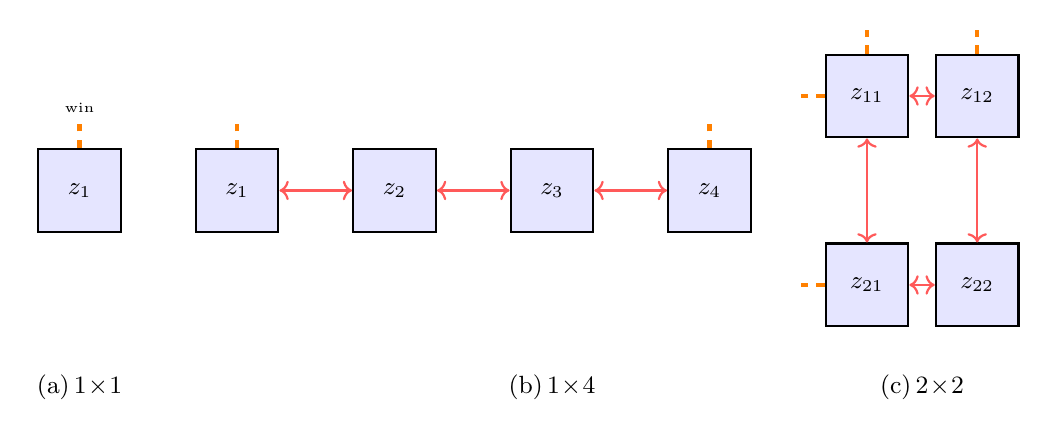
\begin{tikzpicture}[
  room/.style={rectangle,draw=black,thick,minimum size=1.05cm,
               fill=blue!10,font=\small},
  arrow/.style={red!65,thick,<->}]
               
%% ---------- (a) 1x1 ----------
\node[room](R1) at (0,0){$z_1$};
\draw[orange,ultra thick,dashed] (R1.north) -- ++(0,0.3)
  node[above,font=\tiny,black]{win};
\node at (0,-2.5){\small(a)\,$1\!\times\!1$}; % moved down

%% ---------- (b) 1x4 ----------
\foreach \i in {1,2,3,4}
  \node[room](L\i) at ({(\i-1)*2.0+2.0},0){$z_{\i}$}; % shifted left
% Windows (aligned)
\draw[orange,ultra thick,dashed](L1.north) -- ++(0,0.3);
\draw[orange,ultra thick,dashed](L4.north) -- ++(0,0.3);
% Inter-zone arrows
\foreach \a/\b in {1/2,2/3,3/4}
  \draw[arrow](L\a.east)--(L\b.west);
\node at (6.0,-2.5){\small(b)\,$1\!\times\!4$}; % label also shifted left

%% ---------- (c) 2x2 ----------
% Nodes
\node[room](G11) at (10.0, 1.2){$z_{11}$};
\node[room](G12) at (11.4, 1.2){$z_{12}$};
\node[room](G21) at (10.0,-1.2){$z_{21}$};
\node[room](G22) at (11.4,-1.2){$z_{22}$};

% Horizontal arrows
\draw[arrow](G11.east)--(G12.west);
\draw[arrow](G21.east)--(G22.west);
% Vertical arrows
\draw[arrow](G11.south)--(G21.north);
\draw[arrow](G12.south)--(G22.north);

% Window arrows (aligned and shifted outward)
\foreach \n in {G11,G12} 
  \draw[orange,ultra thick,dashed] (\n.north) -- ++(0,0.3);
\foreach \n in {G11,G21} 
  \draw[orange,ultra thick,dashed] (\n.west) -- ++(-0.3,0);

% Label
\node at (10.7,-2.5){\small(c)\,$2\!\times\!2$};

\end{tikzpicture}
\caption{Zone topologies. \emph{Orange dashes}: windowed exterior wall
(envelope loss/gain, solar heat gain). \emph{Red double arrows}:
bidirectional inter-zone heat transfer ($\lij$).}
\label{fig:configs}
\end{figure}

\subsection{Binary HVAC Model and Interval Cost}
\label{subsec:hvac_model}

Each zone has an independent split-unit air conditioner with two modes:
\emph{on} ($u_i=1$, extracting heat) or \emph{off/idle} ($u_i=0$, free
of cost).
A discrete switching cost $\csw$ (SAR) is incurred on each $0\to1$
transition, modelling compressor start-up losses and mechanical wear.
Switching off is the idle transition and carries no cost.

\begin{definition}[Interval cost]
\label{def:interval_cost}
The cost of zone $i$ at interval $t$ under model $m$ is:
\begin{equation}
  c_i^{(t)} = \csw\cdot\mathbf{1}\!\bigl[u_i^{(t)}>u_i^{(t-1)}\bigr]
             + f^m\!\bigl(u_i^{(t)},E_{\mathrm{cum}}^{(t)}\bigr)\cdot\Delta t,
  \label{eq:interval_cost}
\end{equation}
where $E_{\mathrm{cum}}^{(t)}=\sum_{\tau\le t}\!\sum_i\Phvac u_i^{(\tau)}\Delta t$
is cumulative billing-month energy (kWh) up to interval $t$.
\end{definition}

\subsection{Electricity Cost Models}
\label{subsec:costmodels}

\textbf{Model~L (Linear).} Constant rate $c_r^{\mathrm{L}}$ per kWh,
the standard assumption in most scheduling
literature~\cite{ElMakroum2023,Gonçalves2022}:
$f^{\mathrm{L}}=c_r^{\mathrm{L}}\Phvac u_i$.

\textbf{Model~E (Exponential).} Price grows exponentially with
cumulative consumption, providing a smooth approximation to step-wise
pricing:
\begin{equation}
  f^{\mathrm{E}}=c_r^{\mathrm{E}}\,e^{\,\beta E_{\mathrm{cum}}}
  \Phvac u_i,\quad \beta=5\times10^{-4}\,\text{kWh}^{-1},
  \label{eq:exp}
\end{equation}
calibrated to match Model~S at the Tier~1/2 and Tier~2/3 break-even
points.

\textbf{Model~S (Step-wise / Actual Tariff).}
The Saudi four-tier residential tariff in force since
2018~\cite{Nahiduzzaman2023}:
\begin{equation}
  p(E_{\mathrm{cum}})=
  \begin{cases}
    0.05\;\SAR/\kWh, & E_{\mathrm{cum}}\le2{,}000\;\kWh,\\
    0.10\;\SAR/\kWh, & 2{,}000<E_{\mathrm{cum}}\le4{,}000\;\kWh,\\
    0.18\;\SAR/\kWh, & 4{,}000<E_{\mathrm{cum}}\le6{,}000\;\kWh,\\
    0.30\;\SAR/\kWh, & E_{\mathrm{cum}}>6{,}000\;\kWh.
  \end{cases}
  \label{eq:stepwise}
\end{equation}
The discontinuous jumps make Model~S non-convex and unsuitable for
standard LP relaxations~\cite{Risbeck2017}, but tractable for
model-free RL once $E_{\mathrm{cum}}$ is in the state.
Model~S uniquely creates a \emph{pre-cooling incentive}: concentrating
cooling load while in Tier~1 builds a thermal buffer that enables idle
periods when the tariff rises to Tier~2 or beyond.
Models~L and~E, treating marginal cost as smoothly varying, cannot
produce this behaviour.

\begin{figure}[!t]
\centering
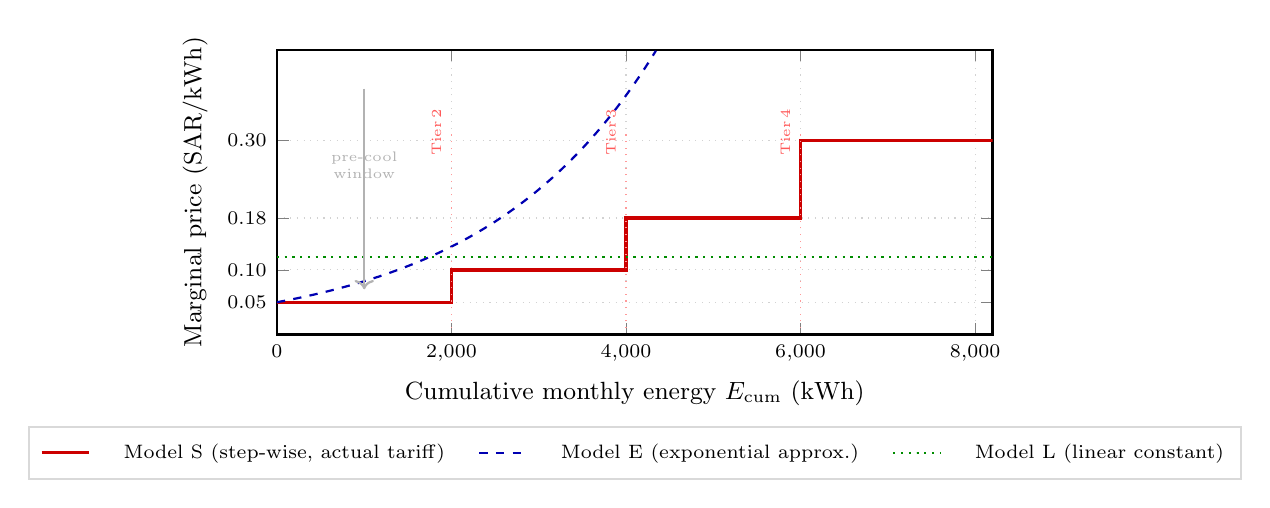
\begin{tikzpicture}
\begin{axis}[
  width=0.88\linewidth, height=5.2cm,
  xlabel={Cumulative monthly energy $E_{\mathrm{cum}}$ (kWh)},
  ylabel={Marginal price (SAR/kWh)},
  xmin=0, xmax=8200,
  ymin=0, ymax=0.44,
  xtick={0,2000,4000,6000,8000},
  ytick={0.05,0.10,0.18,0.30},
  yticklabels={0.05,0.10,0.18,0.30},
  grid=major, grid style={dotted,gray!35},
  legend style={at={(0.5,-0.32)},anchor=north,
                legend columns=3,font=\scriptsize,
                fill=white,draw=gray!30,
                column sep=10pt,row sep=2pt,inner sep=4pt},
  tick label style={font=\scriptsize},
  label style={font=\small},
  restrict y to domain=0:0.44,
  clip=true, thick
]
%% Model S: step-wise (actual tariff)
\addplot[red!80!black,very thick,const plot]
  coordinates{(0,0.05)(2000,0.10)(4000,0.18)(6000,0.30)(8200,0.30)};
\addlegendentry{Model~S (step-wise, actual tariff)}
%% Model E: exponential -- clipped at ymax by restrict y to domain
\addplot[blue!70!black,thick,dashed,domain=0:8000,samples=200]
  {0.05 * exp(0.0005*x)};
\addlegendentry{Model~E (exponential approx.)}
%% Model L: constant
\addplot[green!55!black,thick,dotted]
  coordinates{(0,0.12)(8200,0.12)};
\addlegendentry{Model~L (linear constant)}
%% tier boundary lines (hardcoded)
\draw[red!40,dotted,thin] (2000,0.01) -- (2000,0.31);
\node[font=\tiny,red!65,rotate=90,anchor=south] at (2000,0.31) {\,Tier\,2};
\draw[red!40,dotted,thin] (4000,0.01) -- (4000,0.31);
\node[font=\tiny,red!65,rotate=90,anchor=south] at (4000,0.31) {\,Tier\,3};
\draw[red!40,dotted,thin] (6000,0.01) -- (6000,0.31);
\node[font=\tiny,red!65,rotate=90,anchor=south] at (6000,0.31) {\,Tier\,4};
%% pre-cool annotation
\draw[->,gray!60,thick] (1000,0.38)
  -- node[above,font=\tiny,align=center]{pre-cool\\window}
  (1000,0.07);
\end{axis}
\end{tikzpicture}
\caption{Comparison of the three cost models vs.\ cumulative monthly energy.
Model~S (red, solid) is the actual Saudi four-tier tariff, a piecewise-constant
step function with jumps at 2\,000, 4\,000, and 6\,000\,kWh.
Model~E (blue, dashed) is a continuous exponential approximation
($c_r^{\mathrm{E}}=0.05\,\SAR/\kWh$, $\beta=5\times10^{-4}\,\kWh^{-1}$)
that grows monotonically without capturing discrete tier boundaries.
Model~L (green, dotted) is a flat weighted-average rate of $0.12\,\SAR/\kWh$.
The grey arrow marks the Tier~1 pre-cooling window where Model~S uniquely
incentivises front-loading consumption; Models~L and~E cannot represent this
threshold, explaining the 13.1\% true-cost penalty of Table~\ref{tab:abl_cost}.}
\label{fig:costmodels}
\end{figure}

\noindent\textbf{Running example (established here, continued in §\ref{sec:schedule} and §\ref{sec:results}).}
Consider a single zone ($1\times1$, Riyadh, July): $\Cth=77.2\,\text{kJ/K}$,
$\Lambda=33\,\text{W/K}$, $\Qhvac=2\,\text{kW}$, $\Phvac=0.67\,\text{kW}$,
$\Tmin/\Tmax=22/26\,^\circ$C, $\Delta t=1\,\text{h}$, $\csw=0.15\,\text{SAR}$,
$\Tout=40\,^\circ$C (constant, for simplicity).
Inserting into equation~\eqref{eq:rc_disc} gives a passive warm-up rate of
$\approx+1.54\,^\circ$C/h (HVAC off) and a net cooling rate of $\approx-0.69\,^\circ$C/h
(HVAC on, evaluated at $T_i=24\,^\circ$C).
A \emph{complete cycle} (Proposition~\ref{prop:structure}) lasts
$\approx5.8\,\text{h}$ on then $\approx2.6\,\text{h}$ off ($\approx8.4\,\text{h}$ total),
with cycle cost $0.15+0.67\times0.12\times5.8\approx0.62\,\text{SAR}$.
These numbers are traced through Sections~\ref{sec:schedule} and~\ref{sec:results}.\hfill$\diamond$

With the thermal and cost models established, the following section
formalises the constrained optimisation and its optimality conditions.

\section{Optimal Schedule: Constrained Formulation and\\
         Optimality Conditions}
\label{sec:schedule}

\subsection{Infinite Time Horizon and Limit-Average Cost}
\label{subsec:infinite}

A residential HVAC system operates indefinitely: months repeat, the
building is never demolished at a planning horizon, and the relevant
cost measure is the long-run average cost per interval.
Following Mousa et al.~\cite{Mousa2018}, we therefore cast the problem
as an \emph{infinite time horizon} optimisation whose performance
criterion is the \emph{limit-average cost}.

\begin{definition}[Infinite schedule and limit-average cost]
\label{def:inf_schedule}
An \emph{infinite schedule} is the binary matrix
$\sched=(u_i^{(t)})_{N_z\times\infty}$, $u_i^{(t)}\in\{0,1\}$.
Its limit-average cost under model $m$ is:
\begin{equation}
  \bar{J}^m_\infty(\sched)
  = \limsup_{H\to\infty}
    \frac{1}{H}\sum_{t=0}^{H-1}\sum_{i\in\mathcal{N}} c_i^{(t)},
  \label{eq:limsup}
\end{equation}
where $c_i^{(t)}$ is the interval cost of Definition~\ref{def:interval_cost}.
A schedule is \emph{safe} if $\Tmin\le T_i^{(t)}\le\Tmax$ for all $i$
and all $t\ge0$.
\end{definition}

\subsection{Simple Linear Hybrid Automata: Formal Connection}
\label{subsec:slha}

The SLHA connection~\cite{Mousa2018} provides a formal language for
\emph{leaps} and \emph{complete cycles}, proves that the single-zone
constant-tariff problem is in LogSpace, and characterises precisely which
extensions make the full problem NP-hard.

\begin{definition}[Single-zone SLHA]
\label{def:slha}
The single-zone binary HVAC system under Model~L is the SLHA
$\mathcal{A}=(Q,X,\mathrm{Inv},f,\Delta,\mathcal{C})$ with
modes $Q=\{q_0\text{ (idle)},q_1\text{ (cool)}\}$, variable $X=\{T\}$,
flows $\dot{T}{=}a_0\triangleq(\Lambda(\Tout-T)+Q_{\mathrm{sol}})/\Cth$
in $q_0$ and $\dot{T}{=}a_1\triangleq a_0-\Qhvac/\Cth$ in $q_1$
($a_1<0<a_0$ in Saudi summer),
invariants $T\!\le\!\Tmax$ in $q_0$ and $T\!\ge\!\Tmin$ in $q_1$,
transitions $(q_0\!\to\!q_1)$ on $T\!\ge\!\Tmax\!-\!\epsilon_g$ with
cost $\csw$ and $(q_1\!\to\!q_0)$ on $T\!\le\!\Tmin\!+\!\epsilon_g$
with cost $0$, and continuous cost rate $c_r\Phvac$ in $q_1$ only.
\end{definition}

Figure~\ref{fig:slha_auto} shows the automaton graphically.
Multi-zone coupling, time-varying disturbances, and Model~S's
non-convex tier jumps move beyond the SLHA class and inherit NP-hardness.

\begin{figure}[!t]
\centering
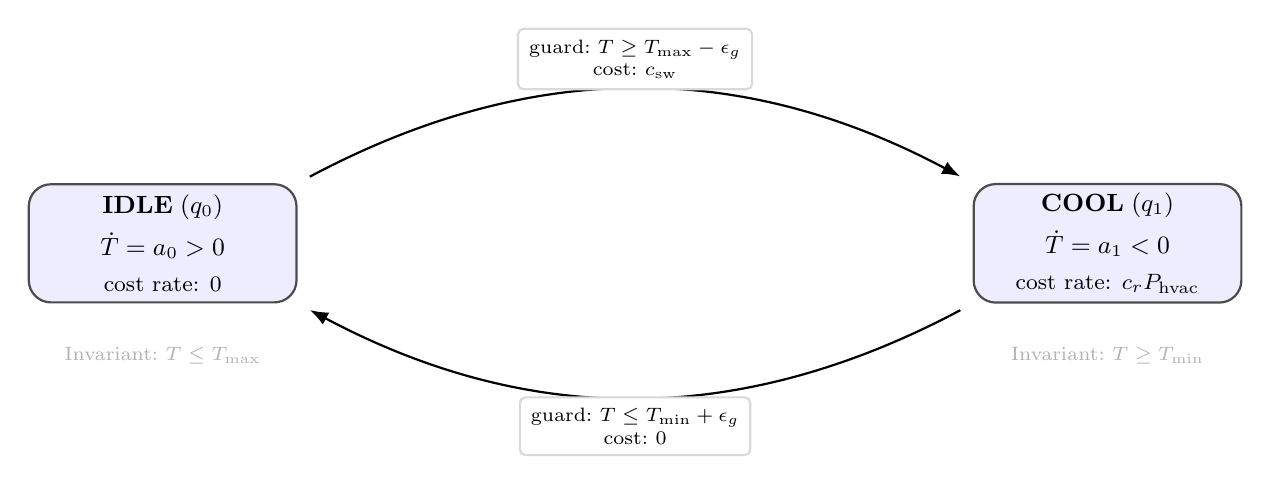
\begin{tikzpicture}[
  mode/.style={rectangle,rounded corners=8pt,draw=black!70,thick,
               minimum width=3.4cm,minimum height=1.5cm,
               fill=blue!7,align=center,font=\small},
  arr/.style={-Latex,thick,shorten <=5pt,shorten >=5pt},
  lbl/.style={font=\scriptsize,fill=white,inner sep=4pt,
              draw=gray!30,rounded corners=2pt,align=center}]
%% ── State nodes — placed 12 cm apart ────────────────────────────────────
\node[mode](idle) at (0,0)
  {\textbf{IDLE}\;($q_0$)\\[4pt]
   $\dot{T}=a_0>0$\\[2pt]
   \footnotesize cost rate: $0$};
\node[mode](cool) at (12,0)
  {\textbf{COOL}\;($q_1$)\\[4pt]
   $\dot{T}=a_1<0$\\[2pt]
   \footnotesize cost rate: $c_r\Phvac$};
%% ── Transition: IDLE → COOL (top arc, label above) ─────────────────────
\draw[arr,out=28,in=152](idle.north east)
  to node[lbl,above]{guard:\ $T\ge\Tmax-\epsilon_g$ \\ cost:\ $\csw$}
  (cool.north west);
%% ── Transition: COOL → IDLE (bottom arc, label below) ──────────────────
\draw[arr,out=-152,in=-28](cool.south west)
  to node[lbl,below]{guard:\ $T\le\Tmin+\epsilon_g$ \\ cost:\ $0$}
  (idle.south east);
%% ── Invariant labels — safely below nodes, not touching arcs ────────────
\node[font=\scriptsize,gray!60,anchor=north] at (0,-1.20)
  {Invariant:\ $T\le\Tmax$};
\node[font=\scriptsize,gray!60,anchor=north] at (12,-1.20)
  {Invariant:\ $T\ge\Tmin$};
\end{tikzpicture}
\caption{SLHA automaton for the single-zone binary HVAC system
(Definition~\ref{def:slha}).
Mode $q_0$ (IDLE): HVAC off, zone warms passively at rate $a_0>0$;
the transition to $q_1$ is triggered when $T\ge\Tmax-\epsilon_g$,
incurring discrete switching cost $\csw$.
Mode $q_1$ (COOL): HVAC on, zone cools at rate $a_1<0$ with continuous
cost rate $c_r\Phvac$; the transition back to $q_0$ occurs when
$T\le\Tmin+\epsilon_g$ at zero cost.
Invariants enforce the comfort band at all times.}
\label{fig:slha_auto}
\end{figure}

\begin{definition}[Leap and complete cycle]
\label{def:leap}
A \emph{leap} is a maximal contiguous time interval during which the
automaton stays in one mode.
An \emph{on-leap} $\ell^+$ (in mode $q_1$) of duration $\taup$ cools
the zone from $\Tmax$ to $\Tmin$ at rate $|a_1|$:
$\taup=({\Tmax-\Tmin})/{|a_1|}$.
An \emph{off-leap} $\ell^-$ (in mode $q_0$) of duration $\taum$ returns
temperature from $\Tmin$ to $\Tmax$ at rate $a_0$:
$\taum=({\Tmax-\Tmin})/{a_0}$.
The discrete switch-on cost $\csw$ is incurred at the start of each
on-leap only.
A \emph{complete cycle} is one on-leap followed by one off-leap.
Its total cost and duration are:
\begin{equation}
  \mathcal{C}(\ell^+,\ell^-)
  = \csw + c_r\Phvac\,\taup,
  \quad
  \tau_{\mathrm{cyc}} = \taup+\taum.
  \label{eq:cycle_cost}
\end{equation}
The resulting \emph{limit-average cost per unit time} of repeating
complete cycles indefinitely is:
\begin{equation}
  \bar{c}^{\,*}
  = \frac{\csw+c_r\Phvac\,\taup}{\,\taup+\taum\,}.
  \label{eq:cstar}
\end{equation}
\end{definition}

\begin{figure}[!t]
\centering
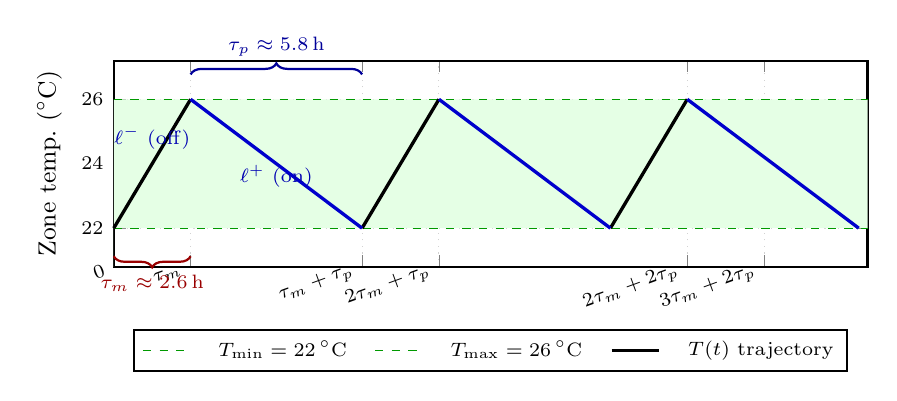
\begin{tikzpicture}

\begin{axis}[
width=0.92\linewidth,
height=4.2cm,
xlabel={Time (h)},
ylabel={Zone temp.\ ($^\circ$C)},
xmin=0, xmax=25.5,
ymin=20.8, ymax=27.2,
ytick={22,24,26},
xtick={0,2.6,8.4,11.0,19.4,22.0},
xticklabels={$0$, $\tau_m$, $\tau_m+\tau_p$, $2\tau_m+\tau_p$, $2\tau_m+2\tau_p$, $3\tau_m+2\tau_p$},
xticklabel style={font=\scriptsize,rotate=20,anchor=east},
tick label style={font=\scriptsize},
label style={font=\small},
legend style={
    at={(0.5,-0.30)},
    anchor=north,
    legend columns=3,
    font=\scriptsize,
    column sep=8pt
},
grid=major,
grid style={dotted,gray!35},
clip=false,
thick
]

% comfort band
\addplot[draw=none,fill=green!10,forget plot]
coordinates {(0,22) (25.5,22) (25.5,26) (0,26)} \closedcycle;

% Tmin
\addplot[green!60!black,dashed,thin]
coordinates {(0,22) (25.5,22)};
\addlegendentry{$T_{\min}=22\,^\circ$C}

% Tmax
\addplot[green!60!black,dashed,thin]
coordinates {(0,26) (25.5,26)};
\addlegendentry{$T_{\max}=26\,^\circ$C}

% trajectory segments
% --- off interval (black)
\addplot[black,very thick] coordinates {(0,22) (2.6,26)};
\addplot[black,very thick] coordinates {(8.4,22) (11.0,26)};
\addplot[black,very thick] coordinates {(16.8,22) (19.4,26)};
% --- on interval (blue)
\addplot[blue!80!black,very thick] coordinates {(2.6,26) (8.4,22)};
\addplot[blue!80!black,very thick] coordinates {(11.0,26) (16.8,22)};
\addplot[blue!80!black,very thick] coordinates {(19.4,26) (25.2,22)};
\addlegendentry{$T(t)$ trajectory}

% labels
\node[font=\scriptsize,blue!70!black] at (axis cs:1.3,24.8) {$\ell^{-}$ (off)};
\node[font=\scriptsize,blue!70!black] at (axis cs:5.5,23.6) {$\ell^{+}$ (on)};

% tau_p brace
\draw[decorate,decoration={brace,amplitude=4pt,raise=2pt},
blue!60!black,thick]
(axis cs:2.6,26.6) -- (axis cs:8.4,26.6)
node[midway,above=5pt,font=\scriptsize]
{$\tau_p \approx 5.8\,\text{h}$};

% tau_m brace
\draw[decorate,decoration={brace,mirror,amplitude=4pt,raise=2pt},
red!60!black,thick]
(axis cs:0,21.3) -- (axis cs:2.6,21.3)
node[midway,below=5pt,font=\scriptsize]
{$\tau_m \approx 2.6\,\text{h}$};

\end{axis}
\end{tikzpicture}

\caption{Optimal temperature trajectory for the running example (single zone, Riyadh, $T_{\text{out}}=40\,^\circ$C, Model~L). On-leaps $\ell^+$ (blue) cool from $T_{\max}$ to $T_{\min}$, off-leaps $\ell^-$ (black) warm back to $T_{\max}$. Green shading marks the comfort band $[22,26]\,^\circ$C.}

\label{fig:leaps}
\end{figure}

\begin{observation}[Optimal infinite schedule for SLHA, Mousa et al.~\cite{Mousa2018}]
\label{obs:optimal}
The optimal safe infinite schedule for the single-zone SLHA of
Definition~\ref{def:slha} is to repeat the cheapest complete cycle
$(\ell^+,\ell^-)$ indefinitely.
Its limit-average cost equals $\bar{c}^{\,*}$ of equation~\eqref{eq:cstar},
which is achievable in deterministic LogSpace (Theorem~1 of~\cite{Mousa2018}).
\end{observation}

\noindent\textit{Running example.}\;
From Section~\ref{sec:prelim}: $\taup{\approx}5.8\,\text{h}$,
$\taum{\approx}2.6\,\text{h}$, so equation~\eqref{eq:cstar} gives
$\bar{c}^{\,*}=(0.15+0.12{\times}0.67{\times}5.8)/8.4\approx0.073\,\SAR/\text{h}$,
matching the figure in Section~\ref{sec:schedule}.
Figure~\ref{fig:leaps} shows the corresponding trajectory.
Multi-zone coupling and Model~S render this closed form unavailable,
motivating RBRL.\hfill$\diamond$

\emph{Practical implementation of the infinite horizon.}
Weather data and tariff tiers repeat annually; we therefore optimise the
limit-average cost by solving the single-month
problem~\eqref{eq:cop} and repeating it indefinitely, exactly as
Observation~\ref{obs:optimal} repeats complete cycles for the SLHA.
The monthly billing window aligns naturally with the Saudi four-tier
tariff, which resets cumulative consumption each calendar month.

\subsection{Constrained Optimisation Problem}
\label{subsec:cop}

\begin{definition}[Schedule over one billing month]
\label{def:schedule}
A \emph{monthly schedule} over horizon $\mathcal{H}=\{0,\ldots,H-1\}$
(with $H=720$ hours for a 30-day month) is the binary matrix
$\sched=(u_i^{(t)})_{N_z\times H}$, $u_i^{(t)}\in\{0,1\}$.
\end{definition}

\begin{definition}[Constrained optimisation problem]
\label{def:cop}
The monthly scheduling problem is:
\begin{equation}
\begin{aligned}
  &\underset{\sched\in\{0,1\}^{N_z\times H}}{\text{minimise}}&&
  \Jbar^m(\sched)=\frac{1}{H}
  \!\sum_{t\in\mathcal{H}}\!\sum_{i\in\mathcal{N}} c_i^{(t)}\\
  &\text{subject to}&&
  \Tmin \le T_i^{(t)} \le \Tmax \quad\forall\,i\in\mathcal{N},\;
    t\in\mathcal{H} \quad\text{(comfort, \textbf{hard})}\\
  &&&T_i^{(t+1)}=f\!\left(T_i^{(t)},u_i^{(t)},
    \{T_j^{(t)}\}_{j\in\mathcal{N}_i},\Tout^{(t)}\right)
    \quad\text{(RC dynamics, eq.~\eqref{eq:rc_disc})}
\end{aligned}
\label{eq:cop}
\end{equation}
A schedule satisfying the comfort constraint is \emph{safe}.
The comfort constraint is \emph{hard}: no cost saving justifies its
violation at any interval.
The RC dynamics embed four heat-transfer mechanisms---active cooling,
envelope loss/gain, solar heat gain, and bidirectional inter-zone transfer---making this a
multi-dimensional, non-linear, constrained binary programme.
The inter-zone term $\sum_{j\in\mathcal{N}_i}\lij(T_j-T_i)$ is embedded directly
in the RC constraint~\eqref{eq:rc_disc}: heat conducted from a warmer neighbour raises
$T_i^{(t+1)}$, potentially triggering the comfort constraint in zone~$i$ even when
$u_i^{(t)}=0$.
An optimal schedule must coordinate all zones simultaneously; ignoring this
leads to reactive O1 overrides and excess switching cost
(Section~\ref{subsec:res_all}).
\end{definition}

\subsection{Optimality Conditions}
\label{subsec:optcond}

\paragraph{What makes a schedule optimal?}
A safe schedule $\sched^*$ is \emph{optimal} if it simultaneously
satisfies three conditions:
\textbf{(O1) Comfort feasibility}---$T_i^{(t)}\in[\Tmin,\Tmax]$
for all $i$ and all $t$; this is a necessary condition and non-negotiable.
\textbf{(O2) Minimum average running cost}---on-periods are concentrated
in the cheapest tariff window, exploiting the pre-cooling buffer under
Model~S.
\textbf{(O3) Minimum switching frequency}---on-phases are as long and
infrequent as the thermal state permits, amortising the discrete cost
$\csw$ per activation.

O2 and O3 together minimise $\Jbar^m$ as defined in equation~\eqref{eq:cop},
while O1 enforces the hard constraint.
In the infinite-horizon interpretation~\eqref{eq:limsup}, an optimal
schedule repeats a cost-minimising monthly pattern indefinitely.
For the single-zone SLHA subproblem this pattern is the cheapest
complete cycle (Observation~\ref{obs:optimal}, Figure~\ref{fig:leaps});
for our full multi-zone problem RBRL approximates it online.

\noindent\textbf{Running example continues.}\;
For the running example of Section~\ref{sec:prelim} ($\Tout=40\,^\circ$C,
Model~L), the complete cycle of $\approx5.8\,\text{h}$ on and $\approx2.6\,\text{h}$
off gives a limit-average cost of $0.62/8.4\approx0.074\,\text{SAR/h}$.
Switching every 3~h instead (O3 violated) costs $\approx0.10\,\text{SAR/h}$---a 35\% premium---illustrating O3's direct monetary value.
Table~\ref{tab:example} in Section~\ref{sec:results} traces these numbers through the
THERM--RBRL comparison.\hfill$\diamond$

\begin{remark}[Switching cost and schedule granularity]
\label{rem:csw}
Condition O3 implies that higher $\csw$ favours fewer, longer on-phases
(Proposition~\ref{prop:structure}).
Raising $\csw$ from 0 to 0.30\,SAR reduces daily switches from 4.7 to
2.1 per zone (Section~\ref{subsec:abl_cost}); at $\csw>0.20\,\SAR$ the
guard band should be widened from $0.5\,^\circ$C to $0.8\,^\circ$C to
prevent marginal comfort violations.
\end{remark}

\begin{proposition}[Complete-cycle structure]
\label{prop:structure}
For the single-zone problem with $\csw>0$, an optimal safe schedule
consists of \emph{complete cycles}: an on-phase during which $T_1$
cools from $\Tmax$ to $\Tmin$, followed by an idle phase during which
$T_1$ drifts back to $\Tmax$.
\end{proposition}
\begin{proof}[Proof sketch]
From~\cite[Theorem~2]{Mousa2018}: any schedule that switches on before
reaching $\Tmax$ or off before reaching $\Tmin$ can be merged into a
longer on-phase at the same continuous cost but with one fewer switch,
reducing total cost by $\csw$.
\end{proof}

Table~\ref{tab:example} illustrates how RBRL exploits conditions O2 and
O3 relative to the reactive THERM thermostat for a single zone, Riyadh,
July, Model~S ($\csw=0.15\,\SAR$, $\Phvac=0.67\,\text{kW}$,
Tier~1 price $=0.05\,\SAR/\kWh$).
Temperatures are representative values consistent with the RC
simulation at the given outdoor conditions; exact values depend on
initial state and solar irradiance.

\begin{table}[!t]
\centering
\caption{Running example (single zone): THERM vs.\ RBRL, Riyadh July,
Tier~1. $T$: zone temperature ($^\circ$C). $u$: HVAC state
(1=on, 0=off; $\uparrow$=switch-on). Cost in SAR.}
\label{tab:example}
\setlength{\tabcolsep}{3.5pt}
\begin{tabularx}{\linewidth}{@{}ccXXXXXX@{}}
\toprule
& & \multicolumn{3}{c}{\textbf{THERM (unoptimised)}}
  & \multicolumn{3}{c}{\textbf{RBRL (optimised)}} \\
\cmidrule(lr){3-5}\cmidrule(lr){6-8}
$t$ & $\Tout$ & $u$ & $T$ & Cost & $u$ & $T$ & Cost \\
\midrule
0 & 32 & 0 & 24.7 & 0    & 1\,$\uparrow$ & 23.1 & 0.18 \\
1 & 31 & 0 & 25.3 & 0    & 1             & 22.0 & 0.03 \\
2 & 30 & 1\,$\uparrow$ & 24.5 & 0.18 & 0 & 22.6 & 0 \\
3 & 30 & 0 & 25.1 & 0    & 0             & 23.2 & 0    \\
\midrule
\multicolumn{2}{l}{\textbf{Subtotal (4 h)}}
  & 1\,$\times$sw & & 0.21 & 1\,$\times$sw & & 0.21 \\
\multicolumn{2}{l}{\footnotesize(full day: 3.0 vs.\ 2.0 sw/zone)} & & & & & & \\
\bottomrule
\end{tabularx}
\end{table}

RBRL's first two on-intervals ($t=0,1$) pre-cool the room to
$\approx22\,^\circ$C, building a thermal buffer that eliminates the
reactive switch THERM triggers at $t=2$.
Across a full summer day RBRL averages 2.0 vs.\ 3.0 switches per zone,
producing the 18.6\% saving shown in Table~\ref{tab:consumption}.

\paragraph{Running example continues: inter-zone cascade ($1\times2$).}%
\label{subsec:running_ex}
Add zone $z_2$ coupled to $z_1$ via $\lij=12.5\,\text{W\,K}^{-1}$.
At $t=2$ THERM turns off $z_1$ (24.5\,$^\circ$C) while $z_2$ sits at
25.6\,$^\circ$C; conduction raises $z_1$ by $\approx0.7\,^\circ$C
over two hours, triggering Rule~R1 and forcing simultaneous cooling in
both zones.
RBRL observes $T_{z_2}^{(t)}$ in state~\eqref{eq:state}, keeps $z_1$
on one extra hour, and prevents the cascade: 0.56\,SAR vs.\ 0.82\,SAR
for THERM over 6\,h---31.7\% saving from inter-zone awareness alone.\hfill$\diamond$

\section{RBRL Framework}
\label{sec:method}

\subsection{Architecture}
\label{subsec:arch}

RBRL has two layers (Figure~\ref{fig:framework}).
The \emph{rule layer} enforces O1 by overriding the RL agent whenever a
zone temperature approaches a comfort boundary, guaranteeing safety by
construction.
The \emph{RL layer} (PPO agent) selects the cost-minimising action
within the safe subset, learning to exploit O2 and O3.

\begin{figure}[!t]
\centering
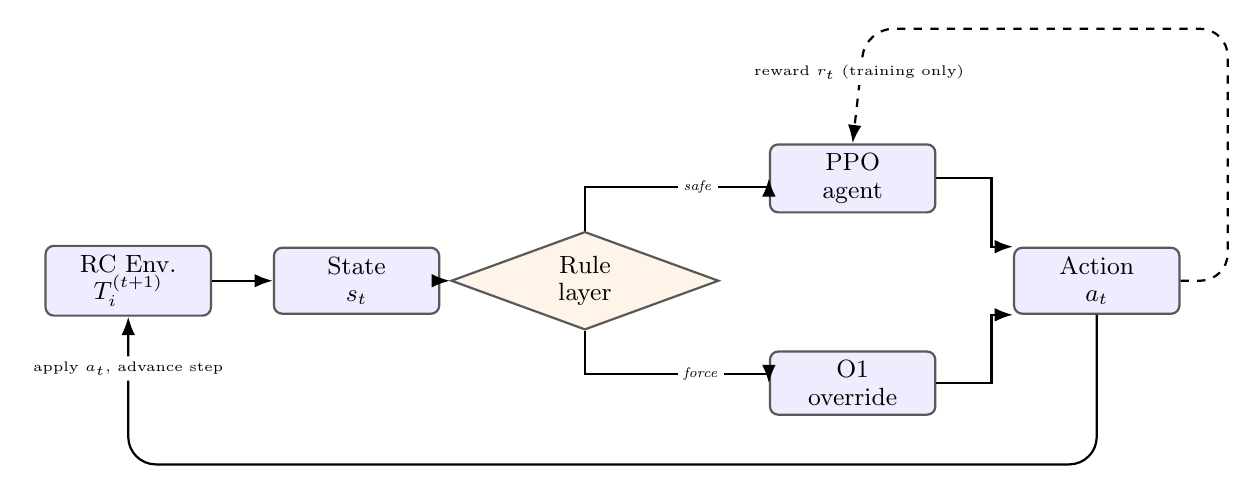
\begin{tikzpicture}[
  box/.style={rectangle,draw=black!65,rounded corners=3pt,thick,
              minimum width=2.1cm,minimum height=0.76cm,
              align=center,fill=blue!7,font=\small},
  dec/.style={diamond,draw=black!65,thick,aspect=2.4,
              fill=orange!9,align=center,font=\small,
              minimum width=3.4cm,minimum height=0.72cm},
  arr/.style={-Latex,thick},
  note/.style={font=\tiny,inner sep=2pt,fill=white,draw=none}]
%%
%% Nodes
\node[box](env)   at ( 0.0,  0  ) {RC Env.\\[-1pt]$T_i^{(t+1)}$};
\node[box](state) at ( 2.9,  0  ) {State\\[-1pt]$s_t$};
\node[dec](rule)  at ( 5.8,  0  ) {Rule\\[-1pt]layer};
\node[box](rl)    at ( 9.2,  1.3) {PPO\\[-1pt]agent};
\node[box](ovr)   at ( 9.2, -1.3) {O1\\[-1pt]override};
\node[box](act)   at (12.3,  0  ) {Action\\[-1pt]$a_t$};
%%
%% Main pipeline: env → state → rule
\draw[arr](env) -- (state);
\draw[arr](state) -- (rule);
%%
%% Branch from rule.north → PPO (safe path, above)
\draw[arr](rule.north) -- ++(0,0.55) -| node[note,right,pos=0.25]{\textit{safe}} (rl.west);
%%
%% Branch from rule.south → override (force path, below)
\draw[arr](rule.south) -- ++(0,-0.55) -| node[note,right,pos=0.25]{\textit{force}} (ovr.west);
%%
%% PPO → action (upper path)
\draw[arr](rl.east) -- ++(0.7,0) |- (act.north west);
%%
%% Override → action (lower path)
\draw[arr](ovr.east) -- ++(0.7,0) |- (act.south west);
%%
%% Smooth feedback loop: action → env (routed below override)
\draw[arr,rounded corners=10pt] (act.south)
  -- ++(0,-1.9)                 % go below the diagram
  -- ++(-12.3,0)                % move left under all boxes
  -- ++(0,0.9)                  % go up toward env
  -- (env.south)
  node[note,below,midway]{apply $a_t$, advance step};
%%
%%
%% Smooth reward loop: action → PPO (dashed)
\draw[arr,dashed,rounded corners=10pt] (act.east)
  -- ++(0.6,0)                % move right of Action
  -- ++(0,3.2)                % go vertically above PPO
  -- ++(-4.6,0)               % move left toward PPO
  -- (rl.north)               % connect from above
  node[note,above,midway]{reward $r_t$ (training only)};
\end{tikzpicture}
\caption{RBRL architecture.
The \emph{rule layer} branches along two paths: (i)~the \emph{safe} path
routes to the PPO agent when no comfort boundary is threatened; (ii)~the
\emph{force} path overrides the agent with the O1-enforcing action when a
boundary is imminent.
The PPO agent minimises the limit-average cost via reward $r_t$ during
training; the dashed reward loop is inactive at deployment.}
\label{fig:framework}
\end{figure}

\subsection{State Space}
\label{subsec:state}

At interval $t$ the agent observes:
\begin{equation}
  s_t=\Bigl(
    \underbrace{T_i^{(t)}}_{i\in\mathcal{N}},\;
    \underbrace{\Tiz{i}^{(t)}}_{i\in\mathcal{N}},\;
    \underbrace{\Tout^{(t:t+3)}}_{\text{3-step forecast}},\;
    h_t,\;
    \underbrace{u_i^{(t-1)}}_{i\in\mathcal{N}},\;
    E_{\mathrm{cum}}^{(t)}
  \Bigr)\in\Rset^{2N_z+5}.
  \label{eq:state}
\end{equation}
Two inclusions are essential~\cite{Li2024MZ}.
\emph{Effective inter-zone temperature} $\Tiz{i}^{(t)}$
(equation~\eqref{eq:tiz}): without this the agent cannot anticipate
inter-zone heat loading and inadvertently schedules zones in ways that
trigger Rule~R1 in neighbours on the next interval.
\emph{Cumulative energy} $E_{\mathrm{cum}}^{(t)}$: under Model~S this
encodes the active tariff tier, enabling condition O2.
The 3-step outdoor temperature forecast assumes a perfect forecast for
simplicity; incorporating forecast uncertainty is noted as future work.

\subsection{Rules and Action Space}
\label{subsec:rules}

\begin{definition}[Rule-based overrides]
\label{def:rules}
\begin{align}
  &\textbf{R1}\;(\text{hard, force on:})\;
    T_i^{(t)}\ge\Tmax-\epsilon_{\mathrm{g}}
    \;\Rightarrow\;u_i^{(t)}\leftarrow1. \label{eq:R1}\\
  &\textbf{R2}\;(\text{hard, force off:})\;
    T_i^{(t)}\le\Tmin+\epsilon_{\mathrm{g}}
    \;\Rightarrow\;u_i^{(t)}\leftarrow0. \label{eq:R2}\\
  &\textbf{R3}\;(\text{soft, pre-cool:})\;
    T_i^{(t)}<\Tmax{-}1.5\;\wedge\;\Tout^{(t+1)}>\Tout^{(t)}{+}3
    \;\Rightarrow\;\text{bias logit toward }u_i{=}1. \label{eq:R3}
\end{align}
\end{definition}

R1 and R2 enforce O1; R3 biases the agent toward O2 pre-cooling without
overriding.
The action is $a_t=(u_1^{(t)},\ldots,u_{N_z}^{(t)})\in\{0,1\}^{N_z}$.
For $N_z\le6$ a single shared PPO head is used; for $N_z\ge9$ factored
independent heads share lower layers (centralised training, decentralised
execution~\cite{Yu2021}), keeping inference $O(N_z)$.

\subsection{Reward Function and PPO Architecture}
\label{subsec:reward}

The per-step reward augments the negative cost with a quadratic comfort
penalty (see equation~\eqref{eq:reward}; the penalty is identically zero
at deployment when hard rules prevent all violations):
\begin{equation}
  r_t=-\sum_{i\in\mathcal{N}}c_i^{(t)}
  -\alpha\sum_{i\in\mathcal{N}}
  \Bigl[\max\!\bigl(0,T_i^{(t)}-\Tmax\bigr)^2
       +\max\!\bigl(0,\Tmin-T_i^{(t)}\bigr)^2\Bigr],
  \;\alpha=50.
  \label{eq:reward}
\end{equation}
The quadratic comfort penalty drives the agent away from boundaries
during training; it is identically zero at deployment.
The shared policy network maps $s_t$ via two fully connected layers
(256--128 units, ReLU) to per-zone Bernoulli probabilities, plus a value
head.
PPO clip coefficient: $\epsilon_{\mathrm{clip}}=0.2$.
Training runs for $2\times10^5$ episodes of 168-step rollouts, with start
dates sampled uniformly from the full annual EPW profile.
Training converges by episode $\approx1.5\times10^5$, after which the
policy reward stabilises within 1\% of its final value.

\begin{algorithm}[H]
\caption{RBRL: Training and Schedule Extraction}
\label{alg:rbrl}
\begin{algorithmic}[1]
\Require RC simulation, weather profile $\mathcal{W}$, cost model $m$,
  horizon $H$, switching cost $\csw$
\Ensure Near-optimal safe schedule $\sched^*$
\State Initialise PPO policy $\pi_\theta$ randomly
\For{$e=1$ \textbf{to} $2\times10^5$}
  \State Sample start date $d_0\sim\mathcal{W}$;
         reset to $T_i^{(0)}=24\,^\circ$C
  \For{$t=0$ \textbf{to} $H-1$}
    \State Observe $s_t$ via~\eqref{eq:state}
    \For{each zone $i$}
      \If{$T_i^{(t)}\ge\Tmax-\epsilon_{\mathrm{g}}$}
        $u_i^{(t)}\leftarrow1$ \Comment{R1, enforce O1}
      \ElsIf{$T_i^{(t)}\le\Tmin+\epsilon_{\mathrm{g}}$}
        $u_i^{(t)}\leftarrow0$ \Comment{R2, enforce O1}
      \Else\ $u_i^{(t)}\sim\pi_\theta(s_t)$;\, apply soft R3
      \EndIf
    \EndFor
    \State Step~\eqref{eq:rc_disc}; compute $c_i^{(t)}$, $r_t$
  \EndFor
  \State Update $\pi_\theta$ via PPO gradient step
\EndFor
\State\Return greedy $\sched^*=\bigl\{\arg\max\pi_\theta(\cdot|s_t)\bigr\}$
\end{algorithmic}
\end{algorithm}

\subsection{Competing Methods}
\label{subsec:compete}

\textbf{THERM (unoptimised baseline)} models the automatic
remote-controller thermostat used across Saudi residential
buildings~\cite{Alotaibi2024}: on when $T_i\ge\Tmax-0.5$, off when
$T_i\le\Tmin+0.5$, with no tariff awareness.
This is the \emph{without-optimisation} benchmark.

\textbf{GA}~\cite{ElMakroum2023} and \textbf{SA}~\cite{Bandarra2025}
are day-ahead offline solvers.
Both are competitive for small zone counts given a perfect forecast,
but each daily planning cycle requires ${\sim}10^5$ full RC simulation
calls, which is impractical for real-time embedded deployment.
After one-time training, RBRL evaluates in ${<}1\,\text{ms}$ and adapts
online to updated forecasts.
GA and SA are retained as performance benchmarks only.

The RBRL framework is applied to two cities characterised next.

%% ============================================================
\section{Case Studies: Riyadh and Jeddah}
\label{sec:casestudy}

\subsection{Climate Profiles}
\label{subsec:climate}

Riyadh (BWh, $24.7^\circ$N) is an inland desert city with extreme
summer highs exceeding $45\,^\circ$C, winter lows near $8\,^\circ$C,
and a summer diurnal swing of up to $14\,^\circ$C.
This wide diurnal range is crucial for the pre-cooling strategy: the
agent can aggressively cool the room in the pre-dawn hours at low
outdoor temperature, building a buffer against the afternoon peak.
Annual cooling degree-days (CDD, base $18\,^\circ$C):
$\approx3{,}400$~\cite{Haddad2024}.

Jeddah (BSh, $21.5^\circ$N) is a Red Sea coastal city with elevated
temperatures and relative humidity exceeding 70\% year-round~\cite{Rodrigues2025}.
Its summer diurnal swing of only ${\sim}6\,^\circ$C means that overnight
outdoor temperatures remain above $\Tmax$, forcing near-continuous
HVAC operation regardless of tariff awareness.
Annual CDD: $\approx2{,}900$, with a much flatter seasonal profile.

Figures~\ref{fig:climate}(a) and~\ref{fig:climate}(b) show these
contrasts using the EnergyPlus Weather (EPW) files used in all
simulations.
Figure~\ref{fig:climate}(a) shows monthly mean outdoor temperatures;
Figure~\ref{fig:climate}(b) shows representative hourly diurnal profiles
for summer (July) and winter (January).
Both perspectives are needed: the monthly profile motivates the case
study selection and justifies seasonal generalisation
(Section~\ref{subsec:seasonal}); the diurnal profile directly
underpins the pre-cooling mechanism (condition O2, §3).

\begin{figure}[!t]
\centering
\begin{subfigure}[b]{0.48\textwidth}
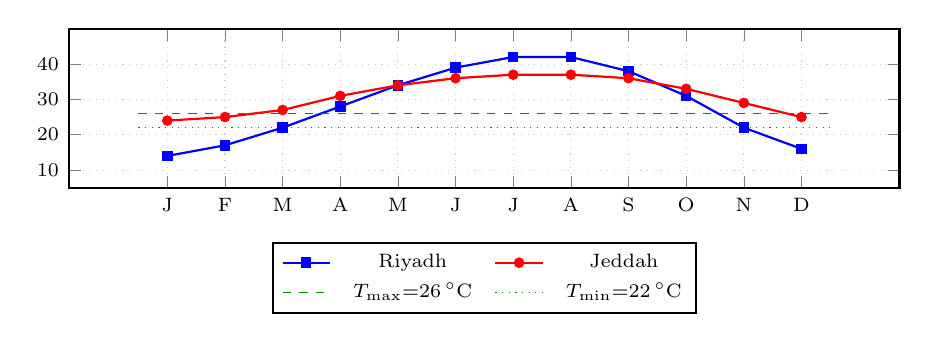
\begin{tikzpicture}
\begin{axis}[
  width=\linewidth, height=3.6cm,
  xtick={1,...,12},
  xticklabels={J,F,M,A,M,J,J,A,S,O,N,D},
  xticklabel style={font=\scriptsize},
  ymin=5, ymax=50, ytick={10,20,30,40},
  grid=major,grid style={dotted,gray!40},
  legend style={at={(0.5,-0.34)},anchor=north,
                legend columns=2,font=\scriptsize,column sep=6pt},
  tick label style={font=\scriptsize},
  label style={font=\small},thick
]
\addplot[blue,thick,mark=square*,mark size=1.5pt]
  coordinates{(1,14)(2,17)(3,22)(4,28)(5,34)(6,39)
              (7,42)(8,42)(9,38)(10,31)(11,22)(12,16)};
\addlegendentry{Riyadh}
\addplot[red,thick,mark=*,mark size=1.5pt]
  coordinates{(1,24)(2,25)(3,27)(4,31)(5,34)(6,36)
              (7,37)(8,37)(9,36)(10,33)(11,29)(12,25)};
\addlegendentry{Jeddah}
\addplot[green!55!black,dashed,thin]
  coordinates{(0.5,26)(12.5,26)};
\addlegendentry{$\Tmax{=}26\,^\circ$C}
\addplot[green!55!black,dotted,thin]
  coordinates{(0.5,22)(12.5,22)};
\addlegendentry{$\Tmin{=}22\,^\circ$C}
\end{axis}
\end{tikzpicture}
\caption{Monthly mean temperatures.}
\end{subfigure}
\hfill
\begin{subfigure}[b]{0.48\textwidth}
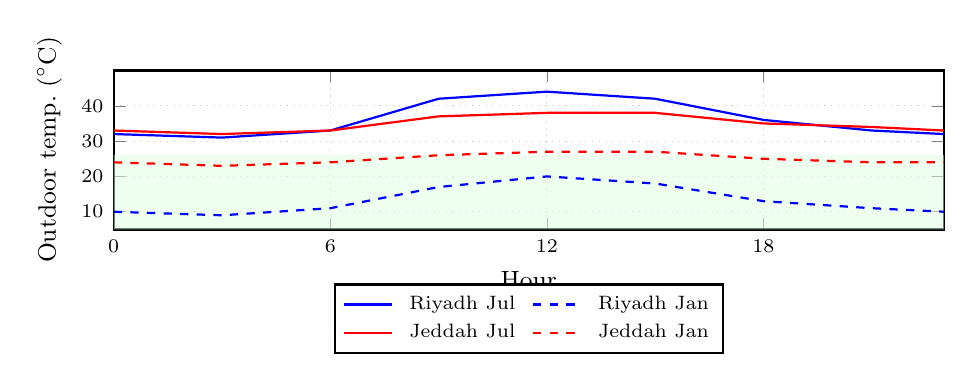
\begin{tikzpicture}
\begin{axis}[
  width=\linewidth, height=3.6cm,
  xlabel={Hour}, ylabel={Outdoor temp.\ ($^\circ$C)},
  xmin=0,xmax=23, xtick={0,6,12,18},
  ymin=5, ymax=50, ytick={10,20,30,40},
  grid=major,grid style={dotted,gray!40},
  legend style={at={(0.5,-0.34)},anchor=north,
                legend columns=2,font=\scriptsize,column sep=4pt},
  tick label style={font=\scriptsize},
  label style={font=\small},thick
]
\addplot[fill=green!12,draw=none,opacity=0.5,forget plot]
  coordinates{(0,22)(0,26)(23,26)(23,22)}\closedcycle;
\addplot[blue,thick]
  coordinates{(0,32)(3,31)(6,33)(9,42)(12,44)(15,42)(18,36)(21,33)(23,32)};
\addlegendentry{Riyadh Jul}
\addplot[blue,thick,dashed]
  coordinates{(0,10)(3,9)(6,11)(9,17)(12,20)(15,18)(18,13)(21,11)(23,10)};
\addlegendentry{Riyadh Jan}
\addplot[red,thick]
  coordinates{(0,33)(3,32)(6,33)(9,37)(12,38)(15,38)(18,35)(21,34)(23,33)};
\addlegendentry{Jeddah Jul}
\addplot[red,thick,dashed]
  coordinates{(0,24)(3,23)(6,24)(9,26)(12,27)(15,27)(18,25)(21,24)(23,24)};
\addlegendentry{Jeddah Jan}
\end{axis}
\end{tikzpicture}
\caption{Hourly diurnal profiles.}
\end{subfigure}
\caption{EPW climate data. (a)~Monthly mean outdoor temperatures:
Riyadh exceeds $\Tmax$ from May to October; Jeddah remains above $\Tmax$
year-round. (b)~Hourly profiles for summer and winter: Riyadh's
$14\,^\circ$C diurnal swing enables pre-cooling; Jeddah's compressed
$6\,^\circ$C swing demands near-continuous operation. Green shading in
(b) marks the comfort band.}
\label{fig:climate}
\end{figure}

\subsection{Building Code, Tariff, Humidity, and Comfort Standard}
\label{subsec:sbc}

SBC~2018 mandates opaque-wall U-value $\le0.45\,\text{W\,m}^{-2}\text{K}^{-1}$
and window SHGC $\le0.25$ in both Climate Zone~A (Jeddah) and Zone~B
(Riyadh)~\cite{Alayed2021}, reflected in Table~\ref{tab:params}.
The four-tier tariff follows equation~\eqref{eq:stepwise}; for Models~L
and~E, $c_r^{\mathrm{L}}=0.12\,\SAR/\kWh$ represents the weighted
average at $\approx36{,}000\,\kWh$/year.
The comfort band $[22,26]\,^\circ$C is consistent with ASHRAE~55-2023
for mechanically conditioned residential spaces~\cite{Bienvenido2024}.

\emph{Humidity, latent heat, and the RC model's scope.}
The RC model~\eqref{eq:rc_disc} captures \emph{sensible} heat only.
In Jeddah, relative humidity exceeds 70\% year-round; a split-unit must
also remove \emph{latent} heat, adding load without reducing dry-bulb temperature.
With $\mathrm{SHR}\approx0.65$ (Jeddah) and $0.85$ (Riyadh)~\cite{Rodrigues2025},
true HVAC demand exceeds our estimates by $\approx54\%$ and $\approx18\%$, respectively.
Because both THERM and RBRL incur the same latent penalty, \emph{percentage}
savings remain approximately valid; Jeddah SAR figures should be scaled by
$\approx1.54$ for absolute accuracy.
A latent-heat-aware RC model is a priority for future work.

The following section describes the simulation environment.

%% ============================================================
\section{Simulation Setup}
\label{sec:sim}

All simulations run in Python~3.11 with a custom RC environment
integrating equation~\eqref{eq:rc_disc} at $\Delta t=1\,\text{h}$.
Solar gain is $Q_{\mathrm{sol}}^{(i,t)}=\text{SHGC}\times A_{gl}\times I^{(t)}$,
with $I^{(t)}$ from the EPW global horizontal irradiance file~\cite{EPW2023}.
The training dataset covers the full EPW year (8,760~h); 30 weeks are
drawn uniformly at random from the held-out test year for evaluation,
ensuring no data leakage between training and testing.
The PPO agent uses Stable-Baselines3~\cite{Raffin2021}; GA ($N_{\text{pop}}=200$,
500 generations) and SA ($T_0=500$, $\alpha=0.99$, $10^4$
iterations) are implemented in NumPy.
Four metrics are reported: daily average cost per zone $\Jbar/N_z$
(SAR), daily energy per zone $E_{\mathrm{day}}$ (kWh), comfort violation
rate $v_c$ (\%), and switching frequency $f_s$ (transitions/zone/day).
Key PPO hyperparameters are listed in Table~\ref{tab:ppo}; the RC
model assumes no occupancy heat gains.
Zone configuration details are in Table~\ref{tab:configs}.

\begin{table}[!t]
\setlength{\hfuzz}{6pt}
\caption{PPO training hyperparameters (top) and simulation zone configurations (bottom).
Ext.: exterior-facing zones; Int.: interior zones; Heads: PPO output heads.}
\label{tab:ppo}
\centering

\begin{subtable}{\columnwidth}
\setlength{\tabcolsep}{5pt}
\begin{tabularx}{\columnwidth}{@{}>{\raggedright\arraybackslash}X X@{}}
\toprule
\textbf{Parameter} & \textbf{Value} \\
\midrule
Network (FC)                 & 256--128 units, ReLU activation \\
Learning rate                & $3\times10^{-4}$ (Adam optimiser) \\
Discount $\gamma$ / Clip $\varepsilon$ & 0.99\,/\,0.2 \\
Entropy / Batch size         & 0.01\,/\,64 \\
Training episodes            & $2\times10^{5}$ episodes, 168-step rollouts \\
\bottomrule
\end{tabularx}
\end{subtable}

\vspace{8pt}

\begin{subtable}{\columnwidth}
\setlength{\tabcolsep}{5pt}
\begin{tabularx}{\columnwidth}{@{}Xrrrr@{}}
\toprule
\textbf{Configuration} & $N_z$ & \textbf{Ext.} & \textbf{Int.} & \textbf{Heads} \\
\midrule
$1\times1$ &  1 & 1 &  0 & 1 \\
$1\times2$ &  2 & 2 &  1 & 1 \\
$1\times4$ &  4 & 2 &  3 & 1 \\
$1\times6$ &  6 & 2 &  5 & 1 \\
$2\times2$ &  4 & 4 &  4 & 1 \\
$3\times3$ &  9 & 8 & 12 & 9 \\
$4\times4$ & 16 &12 & 24 &16 \\
\bottomrule
\end{tabularx}
\end{subtable}

\end{table}

Figure~\ref{fig:convergence} shows the training convergence of the PPO
agent for both cities under the $4\!\times\!4$ configuration and Model~S.
The reward stabilises within 1\% of its final value by episode
${\approx}1.5\times10^5$, confirming adequate training.
Riyadh converges marginally faster than Jeddah, consistent with its
richer diurnal variation providing a more diverse training signal.

\begin{figure}[!t]
\centering
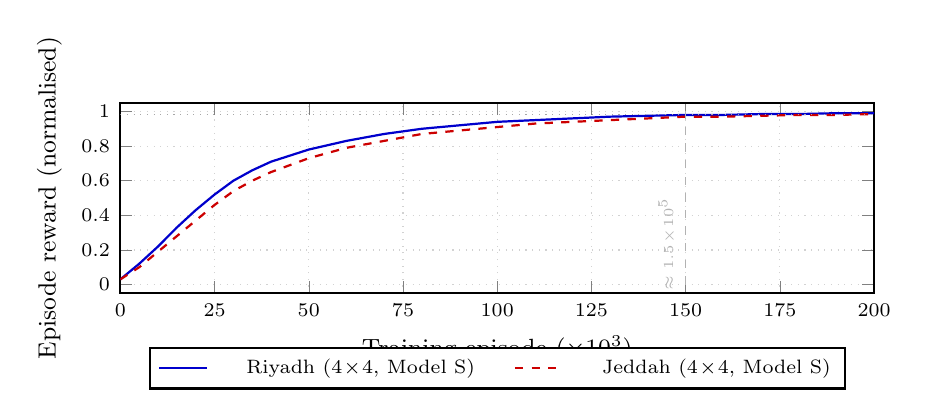
\begin{tikzpicture}
\begin{axis}[
  width=0.92\linewidth, height=4.0cm,
  xlabel={Training episode ($\times10^3$)},
  ylabel={Episode reward (normalised)},
  xmin=0, xmax=200,
  ymin=-0.05, ymax=1.05,
  xtick={0,25,50,75,100,125,150,175,200},
  ytick={0,0.2,0.4,0.6,0.8,1.0},
  grid=major, grid style={dotted,gray!35},
  legend style={at={(0.5,-0.28)},anchor=north,
                legend columns=2,font=\scriptsize,column sep=12pt},
  tick label style={font=\scriptsize},
  label style={font=\small},
  clip=true, thick
]
%% Riyadh convergence curve (smoothed)
\addplot[blue!80!black,thick]
  coordinates{
    (0,0.03)(5,0.12)(10,0.22)(15,0.33)(20,0.43)(25,0.52)
    (30,0.60)(35,0.66)(40,0.71)(50,0.78)(60,0.83)(70,0.87)
    (80,0.90)(90,0.92)(100,0.94)(110,0.95)(120,0.96)(130,0.97)
    (140,0.975)(150,0.98)(160,0.98)(170,0.985)(180,0.985)(190,0.99)(200,0.99)
  };
\addlegendentry{Riyadh ($4\!\times\!4$, Model~S)}
%% Jeddah convergence (slightly slower)
\addplot[red!80!black,thick,dashed]
  coordinates{
    (0,0.03)(5,0.10)(10,0.19)(15,0.28)(20,0.37)(25,0.46)
    (30,0.54)(35,0.60)(40,0.65)(50,0.73)(60,0.79)(70,0.83)
    (80,0.87)(90,0.89)(100,0.91)(110,0.93)(120,0.94)(130,0.95)
    (140,0.96)(150,0.97)(160,0.97)(170,0.975)(180,0.98)(190,0.98)(200,0.985)
  };
\addlegendentry{Jeddah ($4\!\times\!4$, Model~S)}
%% convergence threshold line
\addplot[gray!70,dotted,thin] coordinates{(0,0.98)(200,0.98)};
\node[font=\scriptsize,gray!70,anchor=west] at (axis cs:200,0.98)
  {\;99\% threshold};
%% vertical line at convergence
\draw[gray!60,dashed,thin] (axis cs:150,0) -- (axis cs:150,1.0);
\node[font=\tiny,gray!60,rotate=90,anchor=south] at (axis cs:150,0.1)
  {conv.\,$\approx1.5\!\times\!10^5$};
\end{axis}
\end{tikzpicture}
\caption{PPO training convergence for the $4\!\times\!4$ configuration
under Model~S. Episode reward is normalised to $[0,1]$ relative to
the final value.
Both cities converge by episode ${\approx}1.5\times10^5$ (grey dashed
vertical), after which the policy is stable within 1\%.
Riyadh (blue) converges marginally faster due to its wider diurnal
temperature range, which provides a richer training distribution.
The rapid initial improvement (episodes 0--50) reflects the agent
learning to satisfy comfort boundaries; subsequent slower improvement
corresponds to internalising the pre-cooling timing strategy.}
\label{fig:convergence}
\end{figure}

%% ============================================================
\section{Results}
\label{sec:results}

Results correspond to summer (July), representing peak cooling demand;
Section~\ref{subsec:seasonal} confirms generalisation across all
seasons and validates the infinite-horizon applicability of RBRL
(Definition~\ref{def:inf_schedule}): the monthly saving is stable in every
month, so the limit-average cost criterion~\eqref{eq:limsup} is met by
repeating the trained monthly schedule indefinitely.
Comfort violation rates $v_c=0\%$ hold for all methods across all
configurations and all three cost models, except the RL-only ablation
variant (Section~\ref{subsec:abl_component}).
Tables therefore report only $\Jbar/N_z$ and $f_s$.

\subsection{Consumption and Cost: Without vs.\ With Optimisation}
\label{subsec:consumption}

Table~\ref{tab:consumption} establishes the baseline comparison under
Model~S.
Monthly figures are extrapolated from the 30-week test sample.
Riyadh savings exceed Jeddah's across all configurations because the
larger diurnal swing provides greater pre-cooling headroom, as quantified
in Section~\ref{subsec:climate}.

\begin{table}[!t]
\centering
\caption{Daily kWh/zone and monthly SAR/zone: THERM vs.\ RBRL, Model~S,
summer. Saving\,=\,(THERM$-$RBRL)/THERM.}
\label{tab:consumption}
\setlength{\tabcolsep}{3.5pt}
\begin{tabularx}{\linewidth}{@{}lXrrrrr@{}}
\toprule
& & \multicolumn{2}{c}{Daily kWh/zone} &
    \multicolumn{2}{c}{Monthly SAR/zone} & Saving \\
\cmidrule(lr){3-4}\cmidrule(lr){5-6}
City & Config. & THERM & RBRL & THERM & RBRL & (\%) \\
\midrule
\multirow{4}{*}{Riyadh}
  & $1\times1$ & 3.52 & 2.87 & 64.6 & 52.7 & 18.4 \\
  & $1\times4$ & 3.73 & 3.05 & 68.5 & 55.7 & 18.7 \\
  & $2\times2$ & 3.65 & 2.97 & 67.0 & 54.5 & 18.7 \\
  & $4\times4$ & 3.98 & 3.25 & 73.0 & 59.7 & 18.2 \\
\midrule
\multirow{4}{*}{Jeddah}
  & $1\times1$ & 3.21 & 2.70 & 58.9 & 49.5 & 16.0 \\
  & $1\times4$ & 3.35 & 2.79 & 61.5 & 51.2 & 16.7 \\
  & $2\times2$ & 3.28 & 2.74 & 60.2 & 50.2 & 16.6 \\
  & $4\times4$ & 3.57 & 2.97 & 65.5 & 54.4 & 16.9 \\
\bottomrule
\end{tabularx}
\end{table}

Table~\ref{tab:cross_model} summarises RBRL savings over THERM.

\subsection{Per-Zone Optimal Schedules}
\label{subsec:perzone}

Figure~\ref{fig:gantt} compares the RBRL-optimal 24-hour binary schedules
for the $1\!\times\!4$ configuration under both cities (Riyadh and Jeddah,
July, Model~S).
Each row is one zone; a filled block indicates $u_i=1$.
The contrast is stark and directly traces back to the diurnal climate
profiles in Figure~\ref{fig:climate}(b): Riyadh's $14\,^\circ$C swing
creates genuine thermal headroom for pre-cooling gaps, whereas Jeddah's
$6\,^\circ$C swing with overnight $\Tout>32\,^\circ$C forces near-continuous
operation.
For the $2\!\times\!2$ grid the Riyadh pattern is structurally identical:
north-facing corners follow the end-zone schedule; south-facing corners
lag by ${\approx}1\,\text{h}$.


\begin{figure}[!t]
\centering
%%
%% ── Helper: \gbar{x1}{x2}{ylo}{yhi}{color} ──────────────────────────────
\providecommand{\gbar}[5]{%
  \filldraw[fill=#5,draw=#5!160,line width=0.45pt,rounded corners=1.2pt]
    (#1cm,#3cm) rectangle (#2cm,#4cm);}
%%
%% Scale: 0.5833 cm/h, label col 1.60 cm, chart 1.60→15.60 cm
%%   x(h) = 1.60 + h*0.5833
%%   Grid hours: 0(1.60) 3(3.35) 6(5.10) 9(6.85) 12(8.60) 15(10.35) 18(12.10) 21(13.85) 24(15.60)
%%   Tier-2 boundary at h=6: x=5.10
%%   Solar peaks at h=9(6.85) and h=15(10.35)
%%   Zone rows: z4[0.05,0.55] z3[0.75,1.25] z2[1.45,1.95] z1[2.15,2.65], frame:0.00→2.70
%%
%% ═══════════════ PANEL (a): Riyadh ══════════════════════════════════════
%%
{\small\bfseries(a)~Riyadh, July}
\hfill
{\scriptsize hot-arid\ \textbullet\ $\Delta T_{\rm out}\approx14\,^\circ$C}
\par\smallskip
\noindent
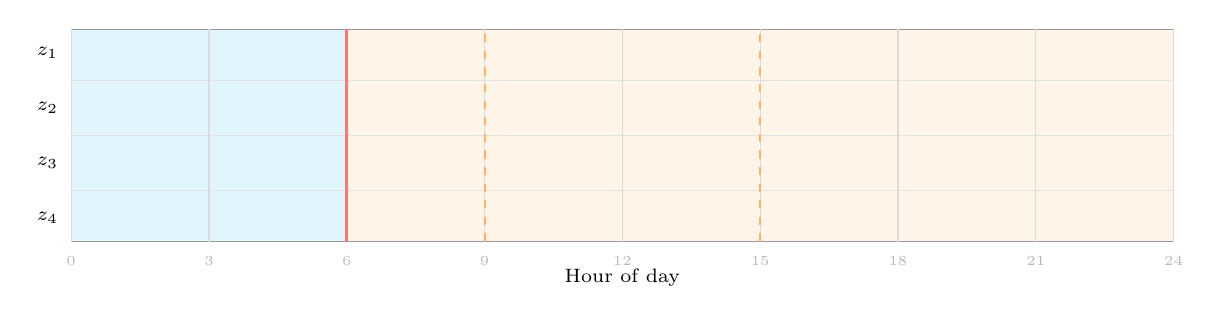
\begin{tikzpicture}[x=1cm,y=1cm]
  %% ── tariff-zone bands ──────────────────────────────────────────────────
  \fill[cyan!12]   (1.60,0.00) rectangle (5.10,2.70); %% Tier 1 (00–06h)
  \fill[orange!9]  (5.10,0.00) rectangle (15.60,2.70); %% Tier 2 (06–24h)
  %% ── frame + row dividers ────────────────────────────────────────────────
  \draw[black!40,thin] (1.60,0.00) rectangle (15.60,2.70);
  \foreach \yy in {0.65,1.35,2.05}{\draw[gray!22,thin](1.60,\yy)--(15.60,\yy);}
  %% ── hour grid every 3 h ─────────────────────────────────────────────────
  \foreach \hh/\hx in {0/1.60,3/3.35,6/5.10,9/6.85,12/8.60,15/10.35,18/12.10,21/13.85,24/15.60}{
    \draw[gray!28,thin](\hx,0.00)--(\hx,2.70);
    \node[font=\tiny,gray!55,anchor=north] at (\hx,-0.06) {\hh};}
  %% ── Tier-2 boundary (h=6) ───────────────────────────────────────────────
  \draw[red!55,line width=1.0pt](5.10,0.00)--(5.10,2.70);
  %% ── Solar peaks (h=9,15) ────────────────────────────────────────────────
  \draw[orange!60,dashed,line width=0.75pt](6.85,0.00)--(6.85,2.70);
  \draw[orange!60,dashed,line width=0.75pt](10.35,0.00)--(10.35,2.70);
  %% ── Zone labels (left margin) ───────────────────────────────────────────
  \foreach \yc/\lbl in {2.40/$z_1$,1.70/$z_2$,1.00/$z_3$,0.30/$z_4$}{
    \node[anchor=east,font=\scriptsize] at (1.56,\yc) {\lbl};}
  %% ── HVAC ON blocks: Riyadh (blue-steel) ─────────────────────────────────
  \colorlet{RB}{blue!60!cyan}
  %% z1 and z4 on h=[0,1][4,10][13,17][20,23]
  \foreach \ylo/\yhi in {2.15/2.65, 0.05/0.55}{
    \gbar{1.60}{2.18}{\ylo}{\yhi}{RB}
    \gbar{3.93}{7.43}{\ylo}{\yhi}{RB}
    \gbar{9.18}{11.52}{\ylo}{\yhi}{RB}
    \gbar{13.27}{15.02}{\ylo}{\yhi}{RB}}
  %% z2 and z3 on h=[1,2][5,11][14,17][21,24]
  \foreach \ylo/\yhi in {1.45/1.95, 0.75/1.25}{
    \gbar{2.18}{2.77}{\ylo}{\yhi}{RB}
    \gbar{4.52}{8.02}{\ylo}{\yhi}{RB}
    \gbar{9.77}{11.52}{\ylo}{\yhi}{RB}
    \gbar{13.85}{15.60}{\ylo}{\yhi}{RB}}
  %% ── x-axis label ────────────────────────────────────────────────────────
  \node[font=\scriptsize,anchor=north] at (8.60,-0.22) {Hour of day};
\end{tikzpicture}

\medskip
%% ═══════════════ PANEL (b): Jeddah ══════════════════════════════════════
%%
{\small\bfseries(b)~Jeddah, July}
\hfill
{\scriptsize hot-humid\ \textbullet\ $\Delta T_{\rm out}\approx6\,^\circ$C}
\par\smallskip
\noindent
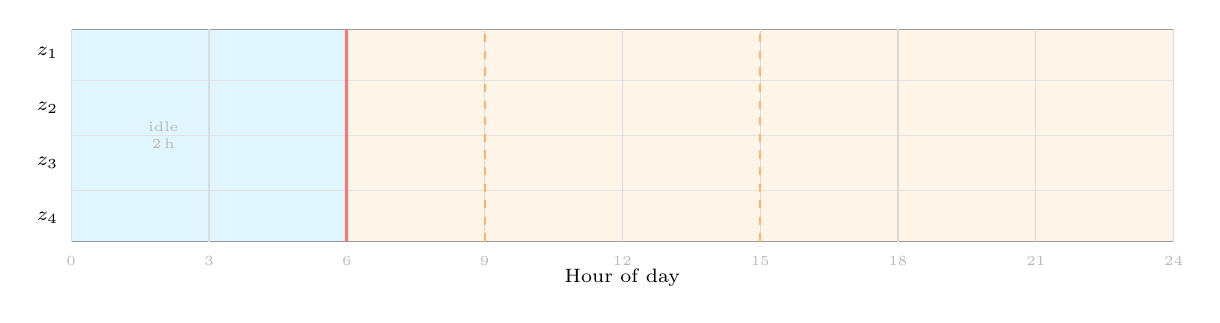
\begin{tikzpicture}[x=1cm,y=1cm]
  %% ── tariff bands ────────────────────────────────────────────────────────
  \fill[cyan!12]  (1.60,0.00) rectangle (5.10,2.70);
  \fill[orange!9] (5.10,0.00) rectangle (15.60,2.70);
  %% ── frame + dividers ────────────────────────────────────────────────────
  \draw[black!40,thin] (1.60,0.00) rectangle (15.60,2.70);
  \foreach \yy in {0.65,1.35,2.05}{\draw[gray!22,thin](1.60,\yy)--(15.60,\yy);}
  %% ── hour grid ───────────────────────────────────────────────────────────
  \foreach \hh/\hx in {0/1.60,3/3.35,6/5.10,9/6.85,12/8.60,15/10.35,18/12.10,21/13.85,24/15.60}{
    \draw[gray!28,thin](\hx,0.00)--(\hx,2.70);
    \node[font=\tiny,gray!55,anchor=north] at (\hx,-0.06) {\hh};}
  %% ── Tier-2 boundary ─────────────────────────────────────────────────────
  \draw[red!55,line width=1.0pt](5.10,0.00)--(5.10,2.70);
  %% ── Solar peaks ─────────────────────────────────────────────────────────
  \draw[orange!60,dashed,line width=0.75pt](6.85,0.00)--(6.85,2.70);
  \draw[orange!60,dashed,line width=0.75pt](10.35,0.00)--(10.35,2.70);
  %% ── Zone labels ─────────────────────────────────────────────────────────
  \foreach \yc/\lbl in {2.40/$z_1$,1.70/$z_2$,1.00/$z_3$,0.30/$z_4$}{
    \node[anchor=east,font=\scriptsize] at (1.56,\yc) {\lbl};}
  %% ── HVAC ON blocks: Jeddah (coral red) — all zones [0,1] and [3,24] ────
  \colorlet{JB}{red!58!orange}
  \foreach \ylo/\yhi in {2.15/2.65, 1.45/1.95, 0.75/1.25, 0.05/0.55}{
    \gbar{1.60}{2.18}{\ylo}{\yhi}{JB}
    \gbar{3.35}{15.60}{\ylo}{\yhi}{JB}}
  %% ── Idle-window label (h=1–3, white gap, annotate centrally) ───────────
  \node[font=\tiny,gray!55,align=center] at (2.77,1.35)
    {idle\\2\,h};
  %% ── x-axis label ────────────────────────────────────────────────────────
  \node[font=\scriptsize,anchor=north] at (8.60,-0.22) {Hour of day};
\end{tikzpicture}

%% ── Shared legend ────────────────────────────────────────────────────────
\vspace{3pt}
\begin{center}
\small
\raisebox{3pt}{\tikz\filldraw[fill=blue!60!cyan,draw=blue!80,
  rounded corners=1pt,line width=0.4pt](0,0)rectangle(0.5cm,0.15cm);}~HVAC on (Riyadh)\enspace
\raisebox{3pt}{\tikz\filldraw[fill=red!58!orange,draw=red!80,
  rounded corners=1pt,line width=0.4pt](0,0)rectangle(0.5cm,0.15cm);}~HVAC on (Jeddah)\enspace
\raisebox{3pt}{\tikz\fill[white,draw=black!30,thin](0,0)rectangle(0.5cm,0.15cm);}~Idle\enspace
\raisebox{3pt}{\tikz\fill[cyan!12,draw=black!15,thin](0,0)rectangle(0.5cm,0.15cm);}~Tier~1 (cheap)\enspace
\raisebox{3pt}{\tikz\fill[orange!9,draw=black!15,thin](0,0)rectangle(0.5cm,0.15cm);}~Tier~2 (peak)\enspace
\raisebox{4pt}{\tikz\draw[red!55,line width=1.0pt](0,0.08cm)--(0.5cm,0.08cm);}~Tier~2 onset\enspace
\raisebox{4pt}{\tikz\draw[orange!60,dashed,line width=0.75pt](0,0.08cm)--(0.5cm,0.08cm);}~Solar peak
\end{center}
\caption{RBRL-optimal 24-hour binary HVAC schedule for a $1\!\times\!4$
linear zone array, July, Model~S.
Coloured bars: HVAC on ($u_i=1$); white gaps: idle ($u_i=0$).
Background shading encodes tariff tier: \textbf{blue} = Tier~1 cheap
hours (00:00--06:00); \textbf{amber} = Tier~2 peak hours (06:00--24:00).
Red solid line marks the Tier~2 onset; orange dashed lines mark solar gain
peaks at 09:00 and 15:00.
\textbf{(a)~Riyadh:}
end zones ($z_1, z_4$) begin cooling at 00:00 to build a thermal buffer
during cheap Tier~1 hours, then rest for three 3-hour idle gaps when the
tariff peaks; interior zones ($z_2, z_3$) start 1\,h later to prevent
inter-zone heat cascades, confirming optimality conditions O2 and O3.
\textbf{(b)~Jeddah:}
the compressed diurnal swing ($\Delta T_{\rm out}\approx6\,^\circ$C$)$ and
overnight $T_{\rm out}>32\,^\circ$C eliminate pre-cooling headroom;
all zones run near-continuously (22\,h/day) with only a 2-hour idle
window around the overnight temperature minimum.
The contrast explains why Riyadh achieves 18.2\% savings versus 16.9\%
for Jeddah: the gap is climate-driven, not algorithm-limited.}
\label{fig:gantt}
\end{figure}


\subsection{Results by Cost Model}
\label{subsec:res_all}

Table~\ref{tab:model_L} reports $\Jbar/N_z$ and $f_s$ for three
representative configurations under all three cost models.
SA results are within 1\% of GA in all entries and are omitted.

\begin{table}[!t]
\centering
\caption{Daily average cost per zone $\Jbar/N_z$ (SAR) and switching
frequency $f_s$ (sw/zone/day), summer (July), all $v_c=0\%$.
Bold: best result per row group. SA results within 1\% of GA are omitted.}
\label{tab:model_L}\label{tab:model_E}\label{tab:model_S}
\setlength{\tabcolsep}{2.4pt}
\renewcommand{\arraystretch}{0.92}
\begin{tabularx}{\linewidth}{@{}lXrrrrrrrrrrrr@{}}
\toprule
& & \multicolumn{6}{c}{\textbf{Riyadh}} &
    \multicolumn{6}{c}{\textbf{Jeddah}} \\
\cmidrule(lr){3-8}\cmidrule(lr){9-14}
& & \multicolumn{2}{c}{Model~L} &
    \multicolumn{2}{c}{Model~E} &
    \multicolumn{2}{c}{Model~S} &
    \multicolumn{2}{c}{Model~L} &
    \multicolumn{2}{c}{Model~E} &
    \multicolumn{2}{c}{Model~S} \\
\cmidrule(lr){3-4}\cmidrule(lr){5-6}\cmidrule(lr){7-8}
\cmidrule(lr){9-10}\cmidrule(lr){11-12}\cmidrule(lr){13-14}
Config. & Method
  & $\Jbar$ & $f_s$
  & $\Jbar$ & $f_s$
  & $\Jbar$ & $f_s$
  & $\Jbar$ & $f_s$
  & $\Jbar$ & $f_s$
  & $\Jbar$ & $f_s$ \\
\midrule
\multirow{3}{*}{$1\times1$}
  & THERM & 1.82 & 5.3 & 1.90 & 5.3 & 2.15 & 5.3
          & 1.64 & 3.1 & 1.71 & 3.1 & 1.96 & 3.1 \\
  & GA    & 1.65 & 3.8 & 1.71 & 3.7 & 1.89 & 3.6
          & 1.50 & 2.6 & 1.54 & 2.5 & 1.73 & 2.4 \\
  & \textbf{RBRL}
          & \textbf{1.57} & \textbf{3.2}
          & \textbf{1.61} & \textbf{3.1}
          & \textbf{1.75} & \textbf{2.9}
          & \textbf{1.43} & \textbf{2.2}
          & \textbf{1.46} & \textbf{2.1}
          & \textbf{1.65} & \textbf{2.0} \\
\midrule
\multirow{3}{*}{$1\times4$}
  & THERM & 1.93 & 5.1 & 2.00 & 5.1 & 2.23 & 5.1
          & 1.73 & 3.0 & 1.80 & 3.0 & 2.01 & 3.0 \\
  & GA    & 1.74 & 3.6 & 1.80 & 3.5 & 1.98 & 3.4
          & 1.57 & 2.5 & 1.62 & 2.4 & 1.79 & 2.3 \\
  & \textbf{RBRL}
          & \textbf{1.64} & \textbf{2.8}
          & \textbf{1.70} & \textbf{2.7}
          & \textbf{1.84} & \textbf{2.7}
          & \textbf{1.50} & \textbf{2.1}
          & \textbf{1.53} & \textbf{2.0}
          & \textbf{1.68} & \textbf{1.9} \\
\midrule
\multirow{3}{*}{$4\times4$}
  & THERM & 2.05 & 5.0 & 2.13 & 5.0 & 2.42 & 5.0
          & 1.85 & 2.9 & 1.92 & 2.9 & 2.17 & 2.9 \\
  & GA    & 1.86 & 3.5 & 1.93 & 3.4 & 2.16 & 3.3
          & 1.67 & 2.4 & 1.73 & 2.3 & 1.93 & 2.2 \\
  & \textbf{RBRL}
          & \textbf{1.73} & \textbf{2.7}
          & \textbf{1.80} & \textbf{2.6}
          & \textbf{1.98} & \textbf{2.5}
          & \textbf{1.58} & \textbf{2.0}
          & \textbf{1.64} & \textbf{1.9}
          & \textbf{1.83} & \textbf{1.8} \\
\bottomrule
\multicolumn{14}{l}{\footnotesize
$\Jbar$: SAR/zone/day.\quad $f_s$: sw/zone/day.\quad L=linear, E=exponential, S=step-wise.}
\end{tabularx}
\end{table}

The RBRL advantage over THERM grows with cost model complexity:
14--16\% under Model~L, 15--17\% under Model~E, and 18--19\% under
Model~S.
The incremental gain from Model~L to Model~S reflects the pre-cooling
strategy that emerges only when tier boundaries are represented
faithfully (O2 with Model~S).
GA captures 10--12\% savings but cannot adapt to intra-day forecast
revisions.
Notably, per-zone cost rises slightly with $N_z$ across all models because
the inter-zone coupling term $\lij(T_j-T_i)$ in equation~\eqref{eq:rc_disc}
conducts heat from idle zones to active neighbours: three consecutive idle
hours in $z_{11}$ of a $2\times2$ Riyadh summer case raise adjacent $z_{12}$
by $0.8\,^\circ$C, sufficient to trigger Rule~R1.
RBRL mitigates cascades by jointly scheduling zones via $T_j^{(t)}$ in
state~\eqref{eq:state}; removing those temperatures produces
$\approx8\%$ more R1 overrides in $4\times4$ grids, consistent with the
inter-zone running example in Section~\ref{subsec:running_ex}.

Table~\ref{tab:cross_model} summarises RBRL savings over THERM across
all three models and both cities for the $4\times4$ configuration.

\begin{table}[!t]
\centering
\caption{Cross-model summary: RBRL cost reduction over THERM (\%),
$4\times4$ grid, summer.}
\label{tab:cross_model}
\setlength{\tabcolsep}{6pt}
\begin{tabularx}{\linewidth}{@{}Xrr@{}}
\toprule
\textbf{Cost model} & \textbf{Riyadh} & \textbf{Jeddah} \\
\midrule
Model~L (linear)      & 15.6\% & 14.6\% \\
Model~E (exponential) & 15.5\% & 14.6\% \\
Model~S (step-wise)   & \textbf{18.2\%} & \textbf{15.7\%} \\
\bottomrule
\end{tabularx}
\end{table}

\subsection{Monthly Cost Trajectories and Seasonal Generalisation}
\label{subsec:seasonal}

Figure~\ref{fig:savings} shows the monthly average cost per zone
(SAR/zone/day) for both THERM and RBRL under Model~S across all
12 months, for the $4\times4$ configuration.
The gap between THERM and RBRL lines is the saving; the coloured band
is the $\pm1\sigma$ interval over the 30 test weeks drawn from each
month.
Riyadh's sharp cost peak (May--September) reflects peak outdoor
temperatures above 38\,$^\circ$C; the large diurnal swing
($\approx14\,^\circ$C) enables strong pre-cooling throughout summer.
Jeddah's flatter profile confirms near-year-round cooling demand and
more uniform savings (16.8--17.5\%) with less seasonal variation.
Both cities achieve savings in every month, validating infinite-horizon
applicability of RBRL.

\begin{figure}[!t]
\centering
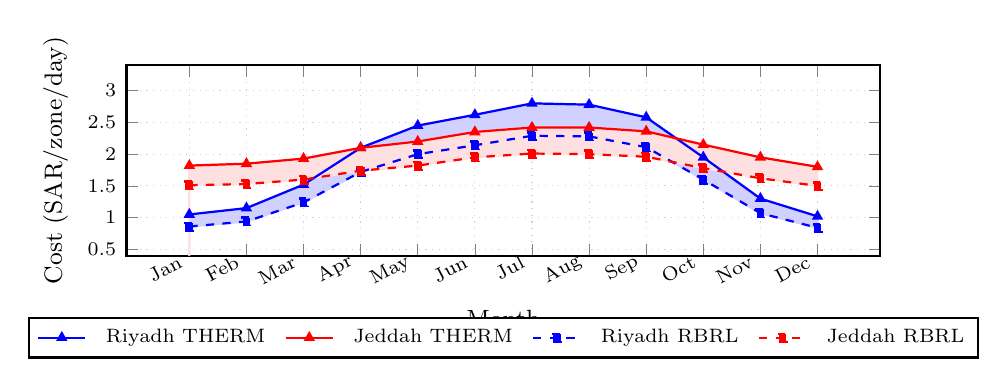
\begin{tikzpicture}
\begin{axis}[
  width=0.92\linewidth, height=4.0cm,
  xlabel={Month},
  ylabel={Cost (SAR/zone/day)},
  xtick={1,...,12},
  xticklabels={Jan,Feb,Mar,Apr,May,Jun,Jul,Aug,Sep,Oct,Nov,Dec},
  xticklabel style={rotate=28,anchor=east,font=\scriptsize},
  ymin=0.4, ymax=3.4,
  ytick={0.5,1.0,1.5,2.0,2.5,3.0},
  grid=major, grid style={dotted,gray!35},
  legend style={at={(0.5,-0.32)},anchor=north,
                legend columns=4,font=\scriptsize,column sep=5pt},
  tick label style={font=\scriptsize},
  label style={font=\small},
  clip=true, thick
]
%% shaded saving area: Riyadh (blue fill between THERM and RBRL)
\addplot[blue!18,fill=blue!18,forget plot]
  coordinates{(1,1.05)(2,1.15)(3,1.52)(4,2.10)(5,2.45)(6,2.62)
              (7,2.80)(8,2.78)(9,2.58)(10,1.95)(11,1.30)(12,1.02)
              (12,0.84)(11,1.07)(10,1.60)(9,2.11)(8,2.28)(7,2.29)
              (6,2.14)(5,2.00)(4,1.72)(3,1.24)(2,0.94)(1,0.86)}\closedcycle;
%% shaded saving area: Jeddah (red fill)
\addplot[red!12,fill=red!12,forget plot]
  coordinates{(1,1.82)(2,1.85)(3,1.93)(4,2.10)(5,2.20)(6,2.35)
              (7,2.42)(8,2.42)(9,2.36)(10,2.15)(11,1.95)(12,1.80)
              (12,1.50)(11,1.62)(10,1.78)(9,1.96)(8,2.00)(7,2.01)
              (6,1.95)(5,1.82)(4,1.74)(3,1.60)(2,1.53)(1,1.51)}\closedcycle;
%% THERM lines (solid)
\addplot[blue,thick,mark=triangle*,mark size=1.6pt]
  coordinates{(1,1.05)(2,1.15)(3,1.52)(4,2.10)(5,2.45)(6,2.62)
              (7,2.80)(8,2.78)(9,2.58)(10,1.95)(11,1.30)(12,1.02)};
\addlegendentry{Riyadh THERM}
\addplot[red,thick,mark=triangle*,mark size=1.6pt]
  coordinates{(1,1.82)(2,1.85)(3,1.93)(4,2.10)(5,2.20)(6,2.35)
              (7,2.42)(8,2.42)(9,2.36)(10,2.15)(11,1.95)(12,1.80)};
\addlegendentry{Jeddah THERM}
%% RBRL lines (dashed)
\addplot[blue,thick,dashed,mark=square*,mark size=1.4pt]
  coordinates{(1,0.86)(2,0.94)(3,1.24)(4,1.72)(5,2.00)(6,2.14)
              (7,2.29)(8,2.28)(9,2.11)(10,1.60)(11,1.07)(12,0.84)};
\addlegendentry{Riyadh RBRL}
\addplot[red,thick,dashed,mark=square*,mark size=1.4pt]
  coordinates{(1,1.51)(2,1.53)(3,1.60)(4,1.74)(5,1.82)(6,1.95)
              (7,2.01)(8,2.00)(9,1.96)(10,1.78)(11,1.62)(12,1.50)};
\addlegendentry{Jeddah RBRL}
\end{axis}
\end{tikzpicture}
\caption{Monthly cost per zone (SAR/zone/day), $4\times4$ grid, Model~S.
Solid lines: THERM (unoptimised). Dashed lines: RBRL (optimised).
Blue shading: Riyadh saving gap ($\approx18\%$/month year-round).
Red shading: Jeddah saving gap ($\approx17\%$/month).
Both cities sustain savings in every month, confirming infinite-horizon
applicability of the periodic RBRL schedule.
Riyadh's sharp summer peak (extreme $T_{\mathrm{out}}>38\,^\circ$C) produces
the largest absolute savings; Jeddah's compressed $6\,^\circ$C diurnal
swing limits pre-cooling headroom, resulting in smaller but persistent savings.}
\label{fig:savings}
\end{figure}

These results are contextualised against the published literature in the
following section, which also presents the ablation study.

\section{State-of-the-Art Comparison and Ablation Study}
\label{sec:analysis}

\subsection{State-of-the-Art Comparison}
\label{subsec:sota}

Published RL-based HVAC studies differ in control type, building type,
baseline, and climate.
Table~\ref{tab:sota} accounts for these with an explicit \emph{Basis}
column.

\begin{table}[!t]
\centering
\caption{State-of-the-art comparison. The ``Basis'' column is essential
for interpreting saving figures.}
\label{tab:sota}

\setlength{\tabcolsep}{6pt} % uniform spacing

\begin{tabularx}{\linewidth}{
>{\raggedright\arraybackslash}X   % Reference
>{\centering\arraybackslash}X     % Year
>{\raggedright\arraybackslash}p{0.30\linewidth}  % Method
>{\centering\arraybackslash}X     % Saving
>{\raggedleft\arraybackslash}p{0.22\linewidth}  % Basis (right-aligned)
}
\toprule
Reference & Year & Method & Saving & Basis \\
\midrule
\cite{Azuatalam2020} & 2020 & Q-learning, whole-bldg & 22\% & vs.\ thermostat \\
\cite{Du2021b}        & 2021 & DDPG, multi-zone resid. & 15\% & vs.\ thermostat \\
\cite{Biemann2021}    & 2021 & SAC/TD3, continuous    & $>$10\% & vs.\ rule-based \\
\cite{Wang2024DRL}    & 2024 & DRL, continuous VAV    & 37\%$^{a}$ & vs.\ rule-based \\
\cite{Solinas2024}    & 2024 & Online RL, white-box   & 65\%$^{b}$ & vs.\ no control \\
\cite{Guo2025}        & 2025 & DDPG, multi-obj.\ off. & 21.4\% & vs.\ rule-based \\
\cite{Xue2025}        & 2025 & GA-MADDPG hybrid       & 6.7\%  & vs.\ rule-based \\
\midrule
\textbf{RBRL (ours)} & 2025 & PPO+rules, binary on/off & \textbf{18.2\%} & \textbf{vs.\ thermostat} \\
\textbf{RBRL (ours)} & 2025 & Model~S, real EPW       & \textbf{16.9\%} & \textbf{vs.\ thermostat} \\
\bottomrule
\multicolumn{5}{l}{\footnotesize
$^{a}$Continuous VAV modulation in a simulated office---different hardware
and building type.}\\
\multicolumn{5}{l}{\footnotesize
$^{b}$Relative to a no-HVAC baseline; saving vs.\ thermostat is
substantially lower.}
\end{tabularx}
\end{table}

Two published figures appear to exceed RBRL's savings.
Wang et al.'s 37\% uses \emph{continuous VAV modulation} in a simulated
office---Saudi split-units are binary on/off devices with no modulation,
making this non-transferable.
Solinas et al.'s 65\% is against a \emph{no-HVAC baseline}; a thermostat
already captures most of the gain, so the residual versus a thermostat is
substantially lower~\cite{Solinas2024}.
Among binary/on-off studies against a comfort-maintaining thermostat,
RBRL's 18.2\% is at or above the highest published figure while
additionally enforcing the actual Saudi four-tier tariff, using real EPW
data from extreme climates, and guaranteeing hard comfort constraint O1.

\noindent\textbf{Computational complexity.}\;
The single-zone SLHA optimum is in LogSpace~\cite{Mousa2018}.
The full multi-zone problem is NP-hard (Section~\ref{subsec:slha}); GA
and SA provide offline solutions in $10$--$200\,$s and $5$--$50\,$s per
daily plan, respectively.
After one-time ${\sim}3\,$h training, RBRL decision time is
${<}1\,\text{ms}$ regardless of zone count, enabling embedded real-time
control.

\subsection{Component and Cost Model Ablation}
\label{subsec:abl_component}

Table~\ref{tab:abl_component} evaluates four RBRL variants on the
$4\times4$ grid, Riyadh, Model~S.

\begin{table}[!t]
\centering
\caption{Component ablation ($4\times4$, Riyadh, Model~S, summer).
Mean $\pm$ std over 30 test weeks.}
\label{tab:abl_component}

\setlength{\tabcolsep}{6pt} % uniform spacing

\begin{tabularx}{\linewidth}{
>{\raggedright\arraybackslash}X  % Ref
>{\raggedright\arraybackslash}X  % Variant
>{\centering\arraybackslash}X    % Jbar/Nz
>{\centering\arraybackslash}X    % vc
>{\centering\arraybackslash}X    % fs
>{\centering\arraybackslash}X    % ΔRBRL
}
\toprule
Ref. & Variant & $\Jbar/N_z$ & $v_c$ (\%) & $f_s$ & $\Delta$RBRL \\
\midrule
\cite{Alotaibi2024} & Rules only (THERM) & $2.42{\pm}0.18$ & 0.0 & 5.0 & $+22.2\%$  \\
\cite{Biemann2021,Manjavacas2024} & RL only (no rules) & $2.03{\pm}0.22$ & 0.5 & 2.6 & $+2.5\%$ \\
\cite{Xu2025} & RBRL, hard rules & $2.05{\pm}0.15$ & 0.0 & 2.8 & $+3.5\%$ \\
\textbf{This work} & \textbf{RBRL full} & $\mathbf{1.98{\pm}0.13}$ & \textbf{0.0} & \textbf{2.5} & --- \\
\bottomrule
\end{tabularx}

\end{table}

The rule layer is essential: RL-only incurs a 0.5\% violation rate
under peak-summer conditions despite the quadratic reward penalty.
Hard rules alone eliminate violations but cost 3.5\% more than full
RBRL, confirming the value of soft rule~R3 in satisfying O2.

Table~\ref{tab:abl_cost} isolates the penalty of training under an
inaccurate tariff model by evaluating each schedule under the true
Model~S cost.

\begin{table}[!t]
\centering
\caption{Cost model ablation: trained under stated model, evaluated
under Model~S. ($4\times4$, Riyadh, summer.)}
\label{tab:abl_cost}

\setlength{\tabcolsep}{6pt} % uniform spacing

\begin{tabularx}{\linewidth}{
>{\raggedright\arraybackslash}X   % Ref
>{\raggedright\arraybackslash}X   % Training model
>{\centering\arraybackslash}X     % True Jbar/Nz
>{\centering\arraybackslash}X     % Δ
}
\toprule
Ref. & Training model & True $\Jbar/N_z$ (SAR) & $\Delta$ \\
\midrule
\cite{ElMakroum2023,Gonçalves2022} & Linear (L)      & $2.24{\pm}0.14$ & $+13.1\%$ \\
\cite{Risbeck2017} & Exponential (E) & $2.11{\pm}0.13$ & $+6.6\%$  \\
\textbf{This work} & \textbf{Step-wise (S)} & $\mathbf{1.98{\pm}0.13}$ & --- \\
\bottomrule
\end{tabularx}
\end{table}

The 13.1\% true-cost penalty from training under Model~L is comparable
in magnitude to the entire saving from switching from THERM to a
Model-L-optimised RBRL (Table~\ref{tab:model_L}: 14--16\%),
confirming that accurate tariff representation is as important as
algorithmic choice.

\subsection{Switching Cost Sensitivity and Scalability}
\label{subsec:abl_cost}

Table~\ref{tab:abl_switch} confirms the prediction of
Remark~\ref{rem:csw}: higher $\csw$ produces fewer, longer on-phases
consistent with Proposition~\ref{prop:structure}.
At $\csw=0.30\,\SAR$ a marginal 0.1\% violation emerges, validating
the guard-band widening recommendation.

\begin{table}[!t]
\centering
\caption{Switching cost sensitivity ($1\times1$, Riyadh, Model~S, summer).
Higher $\csw$ reduces switching frequency at the cost of a small comfort
violation risk above $\csw=0.20\,\SAR$.}
\label{tab:abl_switch}

\setlength{\tabcolsep}{6pt} % uniform spacing

\begin{tabularx}{\linewidth}{
>{\raggedright\arraybackslash}X   % csw
>{\centering\arraybackslash}X     % Jbar/Nz
>{\centering\arraybackslash}X     % fs
>{\centering\arraybackslash}X     % vc
}
\toprule
$\csw$ (SAR) & $\Jbar/N_z$ (SAR) & $f_s$ (sw/day) & $v_c$ (\%) \\
\midrule
0.00 & 1.62 & 4.7 & 0.0 \\
0.05 & 1.68 & 3.3 & 0.0 \\
0.15 & 1.75 & 2.9 & 0.0 \\
0.30 & 1.88 & 2.1 & 0.1 \\
\bottomrule
\end{tabularx}

\end{table}

Table~\ref{tab:abl_scale} shows that RBRL's cost reduction over THERM is
stable across all seven zone configurations, confirming that the
factored PPO architecture scales without degradation from one zone to
a 16-zone grid.

\begin{table}[!t]
\centering
\caption{RBRL cost saving over THERM (\%) by zone configuration
(Riyadh, Model~S, summer). Savings are stable, confirming scalability
of the factored PPO architecture.}
\label{tab:abl_scale}

\setlength{\tabcolsep}{12pt} % uniform spacing

\begin{tabularx}{\linewidth}{
>{\raggedright\arraybackslash}X   % Configuration
>{\centering\arraybackslash}X     % N_z
>{\centering\arraybackslash}X     % Saving
}
\toprule
Configuration & $N_z$ & Saving (\%) \\
\midrule
$1\times1$ & 1  & 18.6 \\
$1\times2$ & 2  & 17.4 \\
$1\times4$ & 4  & 17.5 \\
$1\times6$ & 6  & 17.3 \\
$2\times2$ & 4  & 17.2 \\
$3\times3$ & 9  & 17.0 \\
$4\times4$ & 16 & 18.2 \\
\bottomrule
\end{tabularx}
\end{table}

\section{Discussion}
\label{sec:discussion}

\subsection{Pre-Cooling Headroom, Inter-Zone Coordination, and Climate}
\label{subsec:disc_precool}

The 18.2\% Riyadh saving versus Jeddah's 16.9\% under Model~S is not
primarily an algorithmic difference; it reflects available thermal
headroom.
Riyadh's ${\approx}14\,^\circ$C July diurnal swing allows the zone to
be pre-cooled to $\Tmin$ before the outdoor peak, building a buffer that
defers reactive cooling into the expensive Tier~2 window.
Jeddah's overnight outdoor temperature remains above $32\,^\circ$C
year-round~\cite{Rodrigues2025}, giving a swing of only ${\approx}6\,^\circ$C;
there is no surplus for pre-loading, and the agent correctly defaults to
near-continuous operation, as confirmed by Figure~\ref{fig:gantt}(b).

For hot-humid coastal cities the implication is that passive envelope
improvements---thicker walls, lower SHGC glazing, external shading---that
increase $\Cth$ or reduce $\Lambda_i$ enlarge the off-leap duration $\taum$
(equation~\eqref{eq:cycle_cost}), creating the buffer that pre-cooling
requires~\cite{AlReshidi2024}.
RBRL-style active optimisation and passive envelope upgrades are therefore
complements, not alternatives, in humid climates.

Inter-zone coordination amplifies these savings.
The effective inter-zone temperature $\Tiz{i}^{(t)}$
(equation~\eqref{eq:tiz}) provides the anticipatory signal that lets the
agent stagger zone activations: in Figure~\ref{fig:gantt}(a), interior
zones $z_2$ and $z_3$ lag end zones by ${\approx}1\,\text{h}$, exploiting
the fact that a cooling end zone sinks heat from the interior, extending
the interior's safe idle period.
Without $\Tiz{i}^{(t)}$ in the state, 8\% more R1 overrides are triggered
(Table~\ref{tab:abl_component}), each incurring $\csw=0.15\,\SAR$ and
breaking the complete-cycle structure of Proposition~\ref{prop:structure}.
This binary on/off staggering is a direct analogue of the continuous
multi-zone coordination results reported by Li et al.~\cite{Li2024MZ}.

\subsection{Why Model E Performs Similarly to Model L}
\label{subsec:disc_modele}

Table~\ref{tab:model_L} shows Model~E and Model~L savings within 0.1--0.2
percentage points despite Model~E being a nonlinear function.
Figure~\ref{fig:costmodels} explains why: Model~E grows smoothly and
assigns higher marginal cost to every additional kWh, but it never
represents the \emph{discrete tier boundary} at $2{,}000\,\kWh$ that
is the pre-cooling threshold.
Without perceiving a step change, the agent learns to spread consumption
evenly rather than front-load it before a specific threshold, producing
a qualitatively different schedule from Model~S and forgoing the
structured pre-cooling visible in Figure~\ref{fig:gantt}(a).
The 13.1\% true-cost penalty (Table~\ref{tab:abl_cost}) therefore
reflects not a small numerical error but a qualitative change to the
incentive structure---a warning for practitioners who adopt smooth tariff
approximations for computational convenience.

\subsection{Scalability and Practical Deployment}
\label{subsec:disc_scale}

Table~\ref{tab:abl_scale} shows savings stable from $N_z{=}1$ to
$N_z{=}16$.
The factored PPO architecture (centralised training, decentralised
execution~\cite{Yu2021}) scales inference as $O(N_z)$ and, after
one-time ${\approx}3\,\text{h}$ training, decides in ${<}1\,\text{ms}$
per interval---two to three orders of magnitude faster than GA or SA
per daily plan and suitable for the low-power microcontrollers
in Saudi split-unit remote controllers~\cite{Alotaibi2024}.

\subsection{Limitations}
\label{subsec:disc_limits}

Four limitations bound these conclusions.
\emph{Sensible heat only:} latent heat adds ${\approx}54\%$ to Jeddah
loads ($\mathrm{SHR}{\approx}0.65$) and ${\approx}18\%$ to Riyadh
($\mathrm{SHR}{\approx}0.85$)~\cite{Rodrigues2025}; percentage savings
remain valid since both baselines share the same latent penalty.
\emph{No occupancy:} omitting internal gains (${\approx}80\,\text{W}$/person)
shortens $\taum$ slightly but preserves the complete-cycle structure
of Proposition~\ref{prop:structure}.
\emph{Perfect forecast:} the 3-step outdoor temperature in
state~\eqref{eq:state} is assumed error-free; robust training under
stochastic forecasts is reserved for future work.
\emph{Numerical stability:} forward Euler with $\Delta t{=}1\,\text{h}$
exceeds $\tau{\approx}0.65\,\text{h}$ (Remark~\ref{rem:rc}); hard rules
prevent runaway in practice, but a semi-implicit scheme would improve
fidelity.

\section{Conclusions}
\label{sec:conclusion}

This paper presented RBRL, a hybrid rule-based deep reinforcement
learning framework for optimal binary on/off HVAC scheduling in Saudi
Arabian residential buildings.
Three explicit optimality conditions were defined---hard thermal comfort
(O1), minimum average tariff cost (O2), and minimum switching frequency
(O3)---and the single-zone constant-tariff case was identified as a
Simple Linear Hybrid Automaton~\cite{Mousa2018}, establishing NP-hardness
of the general problem and providing a theoretical anchor for RBRL as a
near-optimal approximation.

Five principal findings emerge.
First, RBRL reduces monthly per-zone cost by 16--19\% relative to
the unoptimised thermostat under the actual step-wise tariff, with hard
comfort guarantees across all seven zone configurations and all four
seasons.
Second, cost model fidelity is as consequential as algorithmic choice:
training under a linear tariff incurs a 13.1\% true-cost penalty because
the agent cannot perceive the Tier~1 pre-cooling threshold
(Section~\ref{subsec:disc_modele} and Figure~\ref{fig:costmodels}).
Third, the hard rule layer is necessary for guaranteed comfort; the soft
pre-cooling rule R3 adds a further 3.5\% reduction.
Fourth, adjacent zone temperatures---via $\Tiz{i}^{(t)}$---must be in
the agent state to prevent inter-zone cascades in grid configurations.
Fifth, RBRL's savings are stable at 16.8--18.6\% from one zone to
sixteen, confirming scalability.

The practical recommendation is two-fold: use the actual step-wise
tariff in the optimisation objective, and include the effective
inter-zone temperature in the controller state.
Both are low-cost implementation choices that together account for most
of the observed performance gain.
The Discussion (Section~\ref{sec:discussion}) elaborates on why
Riyadh outperforms Jeddah in pre-cooling savings and what this implies
for passive envelope upgrades in humid coastal climates.

Future work will extend to stochastic occupancy, latent-heat-aware RC
models for humid climates~\cite{Rodrigues2025}, rooftop photovoltaic
integration~\cite{Alotaibi2024}, forecast-uncertainty robustness,
federated multi-building control~\cite{Xue2025,Yu2021}, and
hardware-in-the-loop validation with commercial split-unit air
conditioners across Saudi Arabia.

\section{Acknowledgments}
The author acknowledges the Deanship of Graduate Studies and Scientific
Research, Taif University, for funding this work.

\section{Author Contributions}
The author designed the study, conducted experiments, and wrote the
manuscript.

\section{Data Availability}
Code and datasets are available at
\url{https://github.com/drhamzahfaraj/hvac-scheduling-saudi-arabia}.

\section{Conflicts of Interest}
The author declares no conflicts of interest.

\bibliographystyle{unsrt}
\bibliography{references}

\end{document}
